\documentclass[10pt,a4paper]{amsart}
\usepackage{amsmath,amssymb,amsthm,graphicx}
\usepackage{amsmath,amssymb,graphicx,xcolor,mathtools,stmaryrd}
\providecommand{\coloneq}{\coloneqq}
\providecommand{\multimapinv}{\mathbin{\rotatebox[origin=c]{180}{$\multimap$}}}
\title{Left and right observational metrics of differential logical relations and compositional function-difference bounds}
\author{Ugo Dal Lago, Naohiko Hoshino, Paolo Pistone}
\date{doi:10.4230/LIPIcs.FSCD.2025.15; CC BY4.0}
\begin{document}
\maketitle
\noindent\textit{Editorial note.} Source https://drops.dagstuhl.de/entities/document/10.4230/LIPIcs.FSCD.2025.15. © Ugo Dal Lago, Naohiko Hoshino and Paolo Pistone, CC BY4.0. Official HTML transcription; original publisher PDF retained.\par\medskip
\noindent\textit{Allowed standard prerequisites (editorial).}\begin{itemize}
\item Quantales, residuation, cartesian closed categories and simply typed lambda calculus. Full author §2–§4 definitions retained; cited background remains in complete source bibliography. Source-local metric and logical-relation constructions are retained as author material.
\end{itemize}\medskip
% BEGIN S2
 
\par\medskip\noindent\textbf{2 From Logical Relations to Differential Logical Relations}\par
 
% BEGIN S2.p1
 
In this section we recall how differential logical relations can be seen as a quantitative generalization of standard logical relations, at the same time highlighting the metric counterparts of qualitative notions like equivalences and preorders. Moreover, we introduce quasi-quasi-metrics as the metric counterpart of quasi-reflexive and transitive relations. For simplicity, we identify lambda terms using the standard $\beta$-equalities throughout this section.\par
 
% END S2.p1
 
% BEGIN S2.SS0.SSS0.P0.SPx1
 
\par\medskip\noindent\textbf{Logical Relations.}\par
 
% BEGIN S2.SS0.SSS0.P0.SPx1.p1
 
The theory of logical relations is well-known and has been exploited in various directions to establish qualitative properties of type systems, like e.g. termination [18], bisimulation [33] or parametricity [30, 21]. The idea is to start from some basic binary relation $\rho_{o}\subseteq o\times o$ over the terms of some ground type $o$. The relation $\rho_{o}$ can then be lifted to a family of binary relations $\rho_{\mathsf{A}}\subseteq\mathsf{A}\times\mathsf{A}$, where $\mathsf{A}$ varies over all simple types constructed starting from $o$ (indeed, one may consider recursive [14], polymorphic [32, 30] or monadic [20] types as well, but we here limit our discussion to simple types). The lifting is defined inductively by:\par
    $\displaystyle(\mathsf{t},\mathsf{t}^{\prime})\in\rho_{\mathsf{A}\times\mathsf{%
B}}$ $\displaystyle\ \iff\ (\mathsf{fst}(\mathsf{t}),\mathsf{fst}(\mathsf{t}^{\prime%
}))\in\rho_{\mathsf{A}}\ \text{and}\ (\mathsf{snd}(\mathsf{t}),\mathsf{snd}(%
\mathsf{t}^{\prime}))\in\rho_{\mathsf{B}},$  ($\land$)    $\displaystyle(\mathsf{t},\mathsf{t}^{\prime})\in\rho_{\mathsf{A}\Rightarrow%
\mathsf{B}}$ $\displaystyle\ \iff\ (\forall\mathsf{s},\mathsf{s}^{\prime}\in\mathsf{A})\ (%
\mathsf{s},\mathsf{s}^{\prime})\in\rho_{\mathsf{A}}\ \Rightarrow\ (\mathsf{t}%
\,\mathsf{s},\mathsf{t^{\prime}}\,\mathsf{s^{\prime}})\in\rho_{\mathsf{B}}.$  ($\Rightarrow$)   
Typically, one wishes to establish a so-called fundamental lemma, stating that well-typed programs $x:\mathsf{A}\vdash\mathsf{t}:\mathsf{B}$ preserve relations. This means that, for any choice of a family of logical relations $\rho_{\mathsf{A}}$ defined as above, one can prove\par
    $\displaystyle(\forall\mathsf{s},\mathsf{s}^{\prime}\in\mathsf{A})\ (\mathsf{s}%
,\mathsf{s}^{\prime})\in\rho_{\mathsf{A}}\ \Rightarrow\ (\mathsf{t}[\mathsf{s}%
/\mathsf{x}],\mathsf{t}[\mathsf{s}^{\prime}/\mathsf{x}])\in\rho_{\mathsf{B}}.$  (Fundamental Lemma)   
Notice that this is equivalent to the instance of reflexivity $(\lambda\mathsf{x}.\mathsf{t},\lambda\mathsf{x}.\mathsf{t})\in\rho_{\mathsf{A}%
\Rightarrow\mathsf{B}}$.\par
 
% END S2.SS0.SSS0.P0.SPx1.p1
 
% BEGIN S2.SS0.SSS0.P0.SPx1.p2
 
Of particular interest are the equivalence relations (that is, those which are reflexive, symmetric and transitive) and the preorders (that is, the reflexive and transitive ones). We here focus on the latter, as we will not consider symmetry in this paper (see Remark 3). A fundamental observation is that the logical relation lifting preserves preorders (and indeed, equivalences): if $\rho_{\mathsf{A}}$ and $\rho_{\mathsf{B}}$ are reflexive and transitive, then $\rho_{\mathsf{A}\times\mathsf{B}}$ and $\rho_{\mathsf{A}\Rightarrow\mathsf{B}}$ can be shown reflexive and transitive as well. The case of the function space crucially relies on the fact that all programs of type $\mathsf{A}\Rightarrow\mathsf{B}$ must preserve relations (or, in other words, that the fundamental lemma holds): as we observed above, the reflexivity condition $(\mathsf{t},\mathsf{t})\in\rho_{\mathsf{A}\Rightarrow\mathsf{B}}$ coincides with the fact that the function $\mathsf{t}$ is relation-preserving; transitivity, instead, can be proved by combining relation-preservation, the reflexivity of $\rho_{\mathsf{A}}$ and the transitivity of $\rho_{\mathsf{B}}$.\par
 
% END S2.SS0.SSS0.P0.SPx1.p2
 
% BEGIN S2.SS0.SSS0.P0.SPx1.p3
 
Any logical relation $\rho\subseteq\mathsf{A}\times\mathsf{A}$ induces an equivalence $\equiv_{\rho}$, called the observational equivalence, where $\mathsf{t}\equiv_{\rho}\mathsf{u}$ iff for all $\mathsf{s}\in\mathsf{A}$, $(\mathsf{s},\mathsf{t})\in\rho$ iff $(\mathsf{s},\mathsf{u})\in\rho$. Intuitively, two terms $\mathsf{t},\mathsf{u}$ are equivalent if the relation $\rho$ cannot distinguish them. For example, if the definition of $\rho_{o}$ on basic types only depends on the values $\mathsf{t}\Rightarrow^{*}\mathsf{v}$ produced by terms, one can usually deduce that terms are indistinguishable from their associated values, that is $\mathsf{t}\equiv_{\rho}\mathsf{v}$. In the absence of symmetry, one obtains two observational preorders $\sqsubseteq^{l}_{\rho},\sqsubseteq^{r}_{\rho}\ \subseteq\mathsf{A}\times%
\mathsf{A}$ defined by:\par
    $\displaystyle\mathsf{s}\ \sqsubseteq^{l}_{\rho}\ \mathsf{t}\ $ $\displaystyle\iff\ (\forall\mathsf{u}\in\mathsf{A})\ (\mathsf{t},\mathsf{u})%
\in\rho\ \Rightarrow\ (\mathsf{s},\mathsf{u})\in\rho,$     $\displaystyle\mathsf{s}\ \sqsubseteq^{r}_{\rho}\ \mathsf{t}\ $ $\displaystyle\iff\ (\forall\mathsf{u}\in\mathsf{A})\ (\mathsf{u},\mathsf{s})%
\in\rho\ \Rightarrow\ (\mathsf{u},\mathsf{t})\in\rho.$    
These preorders satisfy the following useful and easily provable properties:\par
 
% END S2.SS0.SSS0.P0.SPx1.p3
 
% BEGIN Thmtheorem1
 
\par\medskip\noindent\textbf{Proposition 1.}\par
 
% BEGIN Thmtheorem1.p1
 
For any binary relation $\rho\subseteq\mathsf{A}\times\mathsf{A}$ and $c\in\{l,r\}$,\par
  
\par\noindent  (i.) 
% BEGIN S2.I1.i1.p1
 
$\sqsubseteq^{c}_{\rho}\ \supseteq\ \rho$ iff $\rho$ is transitive;\par
 
% END S2.I1.i1.p1
 
 
\par\noindent  (ii.) 
% BEGIN S2.I1.i2.p1
 
$\sqsubseteq^{c}_{\rho}\ \subseteq\ \rho$ iff $\rho$ is reflexive;\par
 
% END S2.I1.i2.p1
 
 
\par\noindent  (iii.) 
% BEGIN S2.I1.i3.p1
 
$\sqsubseteq^{c}_{\rho}\ =\ \rho$ iff $\rho$ is a preorder;\par
 
% END S2.I1.i3.p1
 
 
\par\noindent  (iv.) 
% BEGIN S2.I1.i4.p1
 
The following hold:\par
 
% END S2.I1.i4.p1
 
     $\displaystyle(\forall\mathsf{s},\mathsf{t},\mathsf{u}\in\mathsf{A})\ \mathsf{s%
}\ \sqsubseteq^{l}_{\rho}\ \mathsf{t}\ \land\ (\mathsf{t},\mathsf{u})\in\rho\ %
\Rightarrow\ (\mathsf{s},\mathsf{u})\in\rho,$  (left transitivity)    $\displaystyle(\forall\mathsf{s},\mathsf{t},\mathsf{u}\in\mathsf{A})\ (\mathsf{%
s},\mathsf{t})\in\rho\ \land\ \mathsf{t}\ \sqsubseteq^{r}_{\rho}\ \mathsf{u}\ %
\Rightarrow\ (\mathsf{s},\mathsf{u})\in\rho.$  (right transitivity)   
% END Thmtheorem1.p1
 
% END Thmtheorem1
 
% BEGIN S2.SS0.SSS0.P0.SPx1.p4
 
The reason why we delve into these basic properties of preorders is that we will soon explore their (less trivial!) quantitative counterparts, that arise naturally in the theory of differential logical relations. In particular, the left and right transitivity conditions will correspond to stronger variants of the triangular inequality for metric spaces.\par
 
% END S2.SS0.SSS0.P0.SPx1.p4
 
% BEGIN S2.SS0.SSS0.P0.SPx1.p5
 
Beyond preorders, we are interested in the following weaker notion:\par
 
% END S2.SS0.SSS0.P0.SPx1.p5
 
% BEGIN Thmtheorem2
 
\par\medskip\noindent\textbf{Definition 2 (Quasi-Preorder).}\par
 
% BEGIN Thmtheorem2.p1
 
A relation $\preceq\ \subseteq\mathsf{A}\times\mathsf{A}$ is called a quasi-preorder if it is transitive and (left-)quasi-reflexive, that is, $\mathsf{t}\preceq\mathsf{u}\ \Rightarrow\ \mathsf{t}\preceq\mathsf{t}$.\par
 
% END Thmtheorem2.p1
 
% END Thmtheorem2
 
% BEGIN S2.SS0.SSS0.P0.SPx1.p6
 
Quasi-preorders are obtained by weakening the reflexivity condition of preorders: intuitively, only the points which are smaller than someone are smaller than themselves. One can easily develop a theory of logical relations for quasi-preorders. The sole delicate point is that, in order to let such relations lift to function spaces, one has to slightly modify the relation lifting as follows:\par
    $\displaystyle(\mathsf{t},\mathsf{t}^{\prime})\in\rho_{\mathsf{A}\Rightarrow%
\mathsf{B}}$ $\displaystyle\ \iff\ (\forall\mathsf{s},\mathsf{s}^{\prime}\in\mathsf{A})\ (%
\mathsf{s},\mathsf{s}^{\prime})\in\rho_{\mathsf{A}}\ \Rightarrow\ (\mathsf{t}%
\,\mathsf{s},\mathsf{t^{\prime}}\,\mathsf{s^{\prime}})\in\rho_{\mathsf{B}}\ %
\land\ (\mathsf{t}\,\mathsf{s},\mathsf{t}\,\mathsf{s}^{\prime})\in\rho_{%
\mathsf{B}}.$  ($\Rightarrow^{\mathrm{q}}$)   
Compared to ($\Rightarrow$ \ensuremath{\blacktriangleright} 2), ($\Rightarrow^{\mathrm{q}}$) includes a second clause $(\mathsf{t}\,\mathsf{s},\mathsf{t}\,\mathsf{s}^{\prime})\in\rho_{\mathsf{B}}$ relating the action of $\mathsf{t}$ on both $\mathsf{s}$ and $\mathsf{s}^{\prime}$. With this definition, one can easily check that if $\rho_{\mathsf{A}},\rho_{\mathsf{B}}$ are quasi-preorders, and the fundamental lemma holds, then $\rho_{\mathsf{A}\times\mathsf{B}}$ and $\rho_{\mathsf{A}\Rightarrow\mathsf{B}}$ are quasi-preorders as well.\par
 
% END S2.SS0.SSS0.P0.SPx1.p6
 
% END S2.SS0.SSS0.P0.SPx1
 
% BEGIN S2.SS0.SSS0.P0.SPx2
 
\par\medskip\noindent\textbf{Differential Logical Relations.}\par
 
% BEGIN S2.SS0.SSS0.P0.SPx2.p1
 
We now have all elements to discuss what happens when extending logical relations to a quantitative setting. Rather than considering binary relations $\rho\subseteq\mathsf{A}\times\mathsf{A}$ expressing that a certain property holds for two terms $\mathsf{s},\mathsf{t}$ or not, we will consider ternary relations $\rho\subseteq\mathsf{A}\times\mathcal{Q}_{\mathsf{A}}\times\mathsf{A}$, where $(\mathsf{s},a,\mathsf{t})\in\rho$ indicates that a certain relation holds of $\mathsf{s},\mathsf{t}$ to a certain extent, quantified via $a\in\mathcal{Q}_{\mathsf{A}}$. Here $\mathcal{Q}_{\mathsf{A}}$ is a quantale, an algebraic structure (recalled in the next section) that captures several properties of quantities as expressed by e.g. non-negative real numbers.\par
 
% END S2.SS0.SSS0.P0.SPx2.p1
 
% BEGIN S2.SS0.SSS0.P0.SPx2.p2
 
In fact, just like for standard logical relations, a differential logical relation $\rho_{o}\subseteq o\times\mathcal{Q}_{o}\times o$ on a ground type can be lifted to a family of binary relations $\rho_{\mathsf{A}}\subseteq\mathsf{A}\times\mathcal{Q}_{\mathsf{A}}\times%
\mathsf{A}$ over simple types. First, we define, by induction, the quantales $\mathcal{Q}_{\mathsf{A}\times\mathsf{B}}=\mathcal{Q}_{\mathsf{A}}\times%
\mathcal{Q}_{\mathsf{B}}$ and $\mathcal{Q}_{\mathsf{A}\Rightarrow\mathsf{B}}=\mathsf{A}\Rightarrow(\mathcal{Q%
}_{\mathsf{A}}\rightarrowtriangle\mathcal{Q}_{\mathsf{B}})$, where $\mathcal{Q}_{\mathsf{A}}\rightarrowtriangle\mathcal{Q}_{\mathsf{B}}$ is the quantale of monotone functions, and $\mathsf{A}\Rightarrow\mathcal{Q}_{\mathsf{A}}\rightarrowtriangle\mathcal{Q}_{%
\mathsf{B}}$ is the quantale of functions from the set of closed terms of type $\mathsf{A}$ to $\mathcal{Q}_{\mathsf{A}}\rightarrowtriangle\mathcal{Q}_{\mathsf{B}}$ equipped with the pointwise order. We then define the lifting of $\rho_{o}$ by:\par
    $\displaystyle((\mathsf{t},\mathsf{u}),(a,b),(\mathsf{t}^{\prime},\mathsf{u}^{%
\prime}))\in\rho_{\mathsf{A}\times\mathsf{B}}$ $\displaystyle\iff(\mathsf{t},a,\mathsf{t}^{\prime})\in\rho_{\mathsf{A}}\ \text%
{and}\ (\mathsf{u},b,\mathsf{u}^{\prime})\in\rho_{\mathsf{A}},$     $\displaystyle(\mathsf{t},f,\mathsf{t}^{\prime})\in\rho_{\mathsf{A}\Rightarrow%
\mathsf{B}}$ $\displaystyle\iff(\forall\mathsf{s},\mathsf{s}^{\prime}\in\mathsf{A},\forall a%
\in\mathcal{Q}_{\mathsf{A}})\text{ if }(\mathsf{s},a,\mathsf{s}^{\prime})\in%
\rho_{\mathsf{A}},\text{ then }$      $\displaystyle\mathrel{\phantom{\iff}}(\mathsf{t}\,\mathsf{s},f(\mathsf{s})(a),%
\mathsf{t}\,\mathsf{s^{\prime}})\in\rho_{\mathsf{B}}\text{ and }(\mathsf{t}\,%
\mathsf{s},f(\mathsf{s})(a),\mathsf{t^{\prime}}\,\mathsf{s^{\prime}})\in\rho_{%
\mathsf{B}}.$    
Notice that the definition of $\rho_{\mathsf{A}\Rightarrow\mathsf{B}}$ closely imitates the clause ($\Rightarrow^{\mathrm{q}}$) for quasi-preorders. Also observe that the quantale $\mathcal{Q}_{\mathsf{A}\Rightarrow\mathsf{B}}$ for the function type is itself a set of functions relating terms of type $\mathsf{A}$ and quantities in $\mathcal{Q}_{\mathsf{A}}$ with quantities in $\mathcal{Q}_{\mathsf{B}}$. As we show in Section 5, this definition gives rise to an interpretation of the simply typed $\lambda$-calculus where a fundamental lemma holds under the following form: for all terms $x:\mathsf{A}\vdash\mathsf{t}:\mathsf{B}$ and choice of a family of differential logical relations $\rho_{\mathsf{A}}$ as above, there exists a map ${\mathsf{t}}^{\bullet}:\mathsf{A}\Rightarrow(\mathcal{Q}_{\mathsf{A}}%
\rightarrowtriangle\mathcal{Q}_{\mathsf{B}})$ such that\par
    \[(\forall\mathsf{s},\mathsf{s}^{\prime}\in\mathsf{A},\forall a\in\mathcal{Q}_{%
\mathsf{A}})\ (\mathsf{s},a,\mathsf{s}^{\prime})\in\rho_{\mathsf{A}}\ %
\Rightarrow\ (\mathsf{t}\,\mathsf{s},{\mathsf{t}}^{\bullet}(\mathsf{s})(a),%
\mathsf{t}\,\mathsf{s}^{\prime})\in\rho_{\mathsf{B}}.\]  (fundamental lemma)   
The function ${\mathsf{t}}^{\bullet}$ behaves like some sort of derivative of $\mathsf{t}$: it relates errors in input with errors in output. This connection is investigated in more detail in [9, 29].\par
 
% END S2.SS0.SSS0.P0.SPx2.p2
 
% BEGIN S2.SS0.SSS0.P0.SPx2.p3
 
So far, everything works just as in the standard, qualitative, case. However, the quantitative setting is well visible when we consider the corresponding notions of equivalences and preorders. Recall that an (integral) quantale is, in particular, an ordered monoid $(\mathcal{Q},+,0,\leq)$ of which $0$ is the minimum element. For a differential logical relation $\rho\subseteq\mathsf{A}\times\mathcal{Q}_{\mathsf{A}}\times\mathsf{A}$, reflexivity, symmetry and transitivity translate into the following conditions:\par
    $\displaystyle(\forall\mathsf{t}\in\mathsf{A})\ $ $\displaystyle(\mathsf{t},0,\mathsf{t})\in\rho,$  (reflexivity)    $\displaystyle(\forall\mathsf{t},\mathsf{u}\in\mathsf{A},\forall a\in\mathcal{Q%
}_{\mathsf{A}})\ $ $\displaystyle(\mathsf{t},a,\mathsf{u})\in\rho\ \Rightarrow\ (\mathsf{u},a,%
\mathsf{t})\in\rho,$  (symmetry)    $\displaystyle(\forall\mathsf{s},\mathsf{t},\mathsf{u}\in\mathsf{A},\forall a,b%
\in\mathcal{Q}_{\mathsf{A}})\ $ $\displaystyle(\mathsf{s},a,\mathsf{t})\in\rho\ \land\ (\mathsf{t},b,\mathsf{u}%
)\in\rho\ \Rightarrow\ (\mathsf{s},a+b,\mathsf{u})\in\rho.$  (transitivity)   
It is clear then that equivalence relations translate, in the quantitative setting, into some kind of metric space. Similarly, the quantitative counterpart of preorders are the so-called quasi-metric spaces [19], essentially, metrics without a symmetry condition, indeed a very well-studied class of metrics. In particular, we will show that, similarly to preorders, any ternary relation $\rho\subseteq\mathsf{A}\times\mathcal{Q}_{\mathsf{A}}\times\mathsf{A}$ gives rise to left and right observational quasi-metrics $\rho^{l},\rho^{r}:\mathsf{A}\times\mathsf{A}\to\mathcal{Q}_{\mathsf{A}}$ satisfying properties analogous to those of Proposition 1.\par
 
% END S2.SS0.SSS0.P0.SPx2.p3
 
% BEGIN Thmtheorem3
 
\par\medskip\noindent\textbf{$\blacktriangleright$ Remark 3.}\par
 
% BEGIN Thmtheorem3.p1
 
While in the original definition [11] differential logical relations were symmetric, symmetry was abandoned in all subsequent works. The first reason is that several interesting notions of program difference, like e.g. those arising from incremental computing [9, 6, 1], are not symmetric. A second reason is that the cartesian closure is problematic in presence of both quasi-reflexivity and symmetry [29].\par
 
% END Thmtheorem3.p1
 
% END Thmtheorem3
 
% BEGIN S2.SS0.SSS0.P0.SPx2.p4
 
There is, however, an important point on which differential logical relations differ from standard logical relations: while the former lift preorders well to all simple types, their quantitative counterpart, the quasi-metrics, are not preserved by the higher-order lifting of differential logical relations. Indeed, we observed that an essential ingredient in the lifting of the reflexivity property is the fundamental lemma; yet, in the framework of differential logical relations, the fundamental lemma produces, for any term $\mathsf{t}:\mathsf{A}\Rightarrow\mathsf{B}$, the “reflexivity” condition $(\mathsf{t},{\mathsf{t}}^{\bullet},\mathsf{t})\in\rho_{\mathsf{A}\Rightarrow%
\mathsf{B}}$, which differs from standard reflexivity in that the distance is ${\mathsf{t}}^{\bullet}$ and not the minimum element $0$. This means that the metric structure arising from differential logical relation cannot be that of standard (quasi-)metric spaces. Rather, it must be something close to the partial metric spaces [4, 23], that is, metric spaces in which the condition $d(x,x)=0$ is replaced by the quasi-reflexivity condition $d(x,x)\leq d(x,y)$. We will discuss the connections with partial metric spaces in the next sections.\par
 
% END S2.SS0.SSS0.P0.SPx2.p4
 
% BEGIN S2.SS0.SSS0.P0.SPx2.p5
 
By replacing reflexivity with quasi-reflexivity, we obtain the quantitative counterpart of quasi-preorders, that we call qq-metrics (being “quasi” both in the sense of quasi-metrics, i.e. the rejection of symmetry, and of quasi-preorders, i.e. the weakening of reflexivity).\par
 
% END S2.SS0.SSS0.P0.SPx2.p5
 
% BEGIN Thmtheorem4
 
\par\medskip\noindent\textbf{Definition 4.}\par
 
% BEGIN Thmtheorem4.p1
 
For a set $X$ and a quantale $\mathcal{Q}$, a relation $\rho\subseteq X\times\mathcal{Q}\times X$ is called quasi-quasi-metric (or more concisely qq-metric) if it is transitive and satisfies the condition\par
    $\displaystyle(\forall x,y\in X,\forall a\in\mathcal{Q})\ (x,a,y)\in\rho\ %
\Rightarrow\ (x,a,x)\in\rho.$  (quasi-reflexivity)   
% END Thmtheorem4.p1
 
% END Thmtheorem4
 
% BEGIN S2.SS0.SSS0.P0.SPx2.p6
 
As shown in Section 4, the qq-metrics capture the properties of distances which are preserved by differential logical relations: indeed, the argument showing that the quasi-preorders lift to all simple types scales well to the quantitative setting, showing that a qq-metric on the base types gives rise to qq-metrics on all simple types.\par
 
% END S2.SS0.SSS0.P0.SPx2.p6
 
% BEGIN S2.SS0.SSS0.P0.SPx2.p7
 
The obvious question, however, is: what are these qq-metrics? How are they related to the more standard quasi-metrics and partial metrics? This is what we are going to do in the following section.\par
 
% END S2.SS0.SSS0.P0.SPx2.p7
 
% END S2.SS0.SSS0.P0.SPx2
 
% END S2


% BEGIN S3
 
\par\medskip\noindent\textbf{3 Quasi-Quasi-Metric Spaces}\par
 
% BEGIN S3.p1
 
In this section we use the language of quantale-valued relations to explore the connections between the qq-metrics introduced in the previous section and the more well-established notions of quasi-metric and partial quasi-metric spaces.\par
 
% END S3.p1
 
% BEGIN S3.SS0.SSS0.P0.SPx1
 
\par\medskip\noindent\textbf{Quantale-Valued Relations.}\par
 
% BEGIN S3.SS0.SSS0.P0.SPx1.p1
 
Let us recall that a quantale $\mathcal{Q}$ is a complete lattice $(\mathcal{Q},\sqsubseteq)$ endowed with a continuous monoidal operation $\otimes$, with unit $1$. Here, $\otimes$ being continuous means that both $x\otimes(-)$ and $(-)\otimes x$ preserve arbitrary suprema for all $x\in Q$. A quantale $\mathcal{Q}$ is integral (cf. [22], p. 148) when $1=\top$ and commutative when $\otimes$ is commutative. Suppose $\mathcal{Q}$ is commutative. Given $x,y\in\mathcal{Q}$, their residual is defined as $x\multimap y:=\bigvee\{z\in\mathcal{Q}\mid z\otimes x\sqsubseteq y\}$ where $\sqsubseteq$ is the partial order of $\mathcal{Q}$. Notice that $z\sqsubseteq x\multimap y$ iff $z\otimes x\sqsubseteq y$, and that $(x\multimap y)\otimes x\sqsubseteq y\sqsubseteq x\multimap(y\otimes x)$. A commutative quantale $\mathcal{Q}$ is divisible [23] if for all $x,y\in\mathcal{Q}$, $x\sqsubseteq y$ holds iff $y\otimes(y\multimap x)=x$. Equivalently, $\mathcal{Q}$ is divisible iff, whenever $x\sqsubseteq y$, there exists $z$ such that $x=y\otimes z$. In the following we will use $\mathcal{Q}$ to refer to a commutative, integral and divisible quantale.\par
 
% END S3.SS0.SSS0.P0.SPx1.p1
 
% BEGIN Thmtheorem5
 
\par\medskip\noindent\textbf{Example 5.}\par
 
% BEGIN Thmtheorem5.p1
 
The Lawvere quantale is formed by the non-negative extended reals $[0,+\infty]$ with the reversed order $x\sqsubseteq y:=x\geq y$, and with addition as monoidal operation. Notice that the ordering of quantales is reversed with respect to usual metric intuitions: the “$0$” element is the $\top$, joins correspond to taking $\inf$s, etc.\par
 
% END Thmtheorem5.p1
 
% END Thmtheorem5
 
% BEGIN S3.SS0.SSS0.P0.SPx1.p2
 
Given a quantale $\mathcal{Q}$ and sets $X,Y$, a $\mathcal{Q}$-relation over $X,Y$ is a map $s\colon X\times Y\to\mathcal{Q}$, which can be visualized as a matrix with values in $\mathcal{Q}$. For $\mathcal{Q}$-relations $s,t\colon X\times Y\to\mathcal{Q}$, we write $s\sqsubseteq t$ when $s(x,y)\sqsubseteq t(x,y)$ for all $x\in X$ and $y\in Y$. Given $\mathcal{Q}$-relations $s\colon X\times Y\to\mathcal{Q}$, $t\colon Y\times Z\to\mathcal{Q}$ and $u\colon X\times Z\to\mathcal{Q}$, $w\colon Z\times Y\to\mathcal{Q}$, we define the $\mathcal{Q}$-relations $s\otimes t\colon X\times Z\to\mathcal{Q}$ and $u\multimap s\colon Z\times Y\to\mathcal{Q}$ and $s\multimapinv w\colon X\times Z\to\mathcal{Q}$ via the two operations:\par
    $\displaystyle(s\otimes t)(x,z)$ $\displaystyle=\bigvee_{y\in Y}s(x,y)\otimes t(y,z),$     $\displaystyle(u\multimap s)(z,y)$ $\displaystyle=\bigwedge_{x\in X}u(x,z)\multimap s(x,y),\qquad(s\multimapinv w)%
(x,z)=\bigwedge_{y\in Y}w(z,y)\multimap s(x,y).$    
The monoidal product $\otimes$ and the residuals $\multimap,\multimapinv$ of $\mathcal{Q}$-relations satisfy properties analogous to residuals in $\mathcal{Q}$, e.g. $s\otimes(s\multimap t)\sqsubseteq t$, $(t\multimapinv s)\otimes s\sqsubseteq t$. It is well-known that $\mathcal{Q}$-relations form a category $\mathcal{Q}\textbf{Rel}$ whose objects are sets and such that $\mathcal{Q}\textbf{Rel}(X,Y)$ are the $\mathcal{Q}$-relations from $X$ to $Y$. The operation $s\otimes t$ is the composition operator of this category, while the identities are the relations defined as $\mathbf{1}_{X}(x,x)=1=\top$ and $\mathbf{1}_{X}(x,y\neq x)=\bot$.\par
 
% END S3.SS0.SSS0.P0.SPx1.p2
 
% BEGIN S3.SS0.SSS0.P0.SPx1.p3
 
Finally, for any relation $s\in\mathcal{Q}\mathbf{Rel}(X,X)$, define the relations $\Delta_{1}s,\Delta_{2}s\in\mathcal{Q}\mathbf{Rel}(X,X)$ by $\Delta_{1}s=s\circ\Delta\circ\pi_{1}$ and $\Delta_{2}s=s\circ\Delta\circ\pi_{2}$, that is, $\Delta_{1}s(x,y):=s(x,x)$, $\Delta_{2}s(x,y)=s(y,y)$.\par
 
% END S3.SS0.SSS0.P0.SPx1.p3
 
% END S3.SS0.SSS0.P0.SPx1
 
% BEGIN S3.SS0.SSS0.P0.SPx2
 
\par\medskip\noindent\textbf{Qq- and Quasi-Metric Spaces.}\par
 
% BEGIN S3.SS0.SSS0.P0.SPx2.p1
 
For a relation $s\in\mathcal{Q}\textbf{Rel}(X,X)$, reflexivity $s(x,x)=1$ and transitivity $s(x,z)\otimes s(z,y)\sqsubseteq s(x,y)$ can be written more concisely as $s\sqsupseteq\mathbf{1}_{X}$ and $s\otimes s\sqsubseteq s$. A relation $s$ satisfying both such properties is called a quasi-(pseudo)metric (or a hemi-metric) over $X$ (with values in $\mathcal{Q}$). The “pseudo” prefix stands for the fact that the usual separation property $s(x,y)=1\Rightarrow x=y$ needs not hold. As we do not investigate separation here, all metric notions discussed in the rest of the paper are to be understood as implicitly “pseudo”.\par
 
% END S3.SS0.SSS0.P0.SPx2.p1
 
% BEGIN S3.SS0.SSS0.P0.SPx2.p2
 
The following construction generalizes the observational preorders to $\mathcal{Q}$-relations:\par
 
% END S3.SS0.SSS0.P0.SPx2.p2
 
% BEGIN Thmtheorem6
 
\par\medskip\noindent\textbf{Proposition 6.}\par
 
% BEGIN Thmtheorem6.p1
 
For all $s\in\mathcal{Q}\mathbf{Rel}(X,X)$, the relations $s^{l}:=s\multimapinv s,s^{r}:=s\multimap s\in\mathcal{Q}\mathbf{Rel}(X,X)$ are quasi-metrics and, for $c\in\{l,r\}$, the following hold:\par
  
\par\noindent  (i.) 
% BEGIN S3.I1.i1.p1
 
$s^{c}\sqsupseteq s$ iff $s$ is transitive;\par
 
% END S3.I1.i1.p1
 
 
\par\noindent  (ii.) 
% BEGIN S3.I1.i2.p1
 
$s^{c}\sqsubseteq s$ iff $s$ is reflexive;\par
 
% END S3.I1.i2.p1
 
 
\par\noindent  (iii.) 
% BEGIN S3.I1.i3.p1
 
$s^{c}=s$ iff $s$ is a quasi-metric;\par
 
% END S3.I1.i3.p1
 
 
\par\noindent  (iv.) 
% BEGIN S3.I1.i4.p1
 
$s^{l}\otimes s\sqsubseteq s$ and $s\otimes s^{r}\sqsubseteq s$, that is, the following hold:\par
 
% END S3.I1.i4.p1
 
     $\displaystyle(\forall x,y,z\in X)\ \ s^{l}(x,z)\otimes s(z,y)$ $\displaystyle\sqsubseteq s(x,y),$  (left transitivity)    $\displaystyle(\forall x,y,z\in X)\ \ s(x,z)\otimes s^{r}(z,y)$ $\displaystyle\sqsubseteq s(x,y).$  (right transitivity)   
% END Thmtheorem6.p1
 
% END Thmtheorem6
 
% BEGIN S3.SS0.SSS0.P0.SPx2.p3
 
We call the quasi-metrics $s^{l},s^{r}$ the left and right observational quasi-metric of $s$.\par
 
% END S3.SS0.SSS0.P0.SPx2.p3
 
% BEGIN S3.SS0.SSS0.P0.SPx2.p4
 
Qq-metrics correspond to $\mathcal{Q}$-relations $s\in\mathcal{Q}\mathbf{Rel}(X,X)$ satisfying transitivity $s\otimes s\sqsubseteq s$ and quasi-reflexivity $s\sqsubseteq\Delta_{1}s$ (i.e. $s(x,y)\sqsubseteq s(x,x)$). From transitivity, we deduce that, for a qq-metric $s$, both $s^{l},s^{r}\sqsupseteq s$ hold, that is, the observational quasi-metrics yield tighter distances than $s$. This implies that left and right transitivity read as stronger forms of the triangular inequality. In particular, the following alternative characterization of qq-metrics holds:\par
 
% END S3.SS0.SSS0.P0.SPx2.p4
 
% BEGIN Thmtheorem7
 
\par\medskip\noindent\textbf{Proposition 7.}\par
 
% BEGIN Thmtheorem7.p1
 
For any quasi-reflexive $s\in\mathcal{Q}\mathbf{Rel}(X,X)$, $s$ is a qq-metric iff there exists a quasi-metric $q\sqsupseteq s$ such that either $s\otimes q\sqsubseteq s$ or $q\otimes s\sqsubseteq s$ holds. Furthermore, when $s$ is a qq-metric, both $s^{l}$ and $s^{r}$ are quasi-metrics.\par
 
% END Thmtheorem7.p1
 
% END Thmtheorem7
 
% END S3.SS0.SSS0.P0.SPx2
 
% BEGIN S3.SS0.SSS0.P0.SPx3
 
\par\medskip\noindent\textbf{Qq- and Partial Metric Spaces.}\par
 
% BEGIN S3.SS0.SSS0.P0.SPx3.p1
 
Let us now discuss the connection with partial metric spaces. We here consider the non-symmetric variant of the partial metric spaces from [4], called partial quasi-metric spaces (PQM) [24]. As we anticipated, these are metrics $p$ for which the usual reflexivity condition $p(x,x)=1$ is replaced by the weaker quasi-reflexivity condition $p(x,x)\sqsupseteq p(x,y)$. However, unlike the qq-metrics just discussed, PQMs satisfy a stronger transitivity condition. When $\mathcal{Q}=[0,+\infty]$ is the Lawvere quantale, this condition reads as\par
    \[p(x,z)+p(z,y)-p(z,z)\sqsupseteq p(x,y).\]  (strong transitivity in $[0,+\infty]$)   
The idea is that the self-distance of the central term $z$ is “subtracted”. For a general quantale $\mathcal{Q}$, this becomes:\par
    \[p(x,z)\otimes(p(z,z)\multimap p(z,y))\sqsubseteq p(x,y).\]  (strong transitivity)   
% END S3.SS0.SSS0.P0.SPx3.p1
 
% BEGIN S3.SS0.SSS0.P0.SPx3.p2
 
Define the relations $\Theta^{l}_{s},\Theta^{r}_{s}\in\mathcal{Q}\mathbf{Rel}(X,X)$ by $\Theta^{l}_{s}(x,y)=s(y,y)\multimap s(x,y)$ and $\Theta^{r}_{s}(x,y)=s(x,x)\multimap s(x,y)$. A PQM can be thus more concisely be defined as a relation $s\in\mathcal{Q}\mathbf{Rel}(X,X)$ satisfying $s\sqsubseteq\Delta_{1}s$ and $s\otimes\Theta^{r}_{s}\sqsubseteq s$. Notice that strong transitivity $s\otimes\Theta^{r}_{s}\sqsubseteq s$ looks similar to the right transitivity $s\otimes q^{r}_{s}\sqsubseteq s$. Indeed, the following result relates the relations $\Theta^{c}_{s}$ and $s^{c}$:\par
 
% END S3.SS0.SSS0.P0.SPx3.p2
 
% BEGIN Thmtheorem8
 
\par\medskip\noindent\textbf{Proposition 8.}\par
 
% BEGIN Thmtheorem8.p1
 
For all $s\in\mathcal{Q}\mathbf{Rel}(X,X)$ and $c\in\{l,r\}$, $s^{c}\sqsubseteq\Theta^{c}_{s}$. Moreover, if $s$ is quasi-reflexive, $\Theta^{c}_{s}\sqsubseteq s^{c}$ holds iff $\Theta^{c}_{s}$ is a quasi-metric iff $s$ is a partial quasi-metric.\par
 
% END Thmtheorem8.p1
 
% END Thmtheorem8
 
% BEGIN S3.SS0.SSS0.P0.SPx3.p3
 
The result above suggests that the partial quasi-metrics can be seen as limit cases of the qq-metrics, namely those for which the quasi-metric $s^{r}(x,y)$ can be written under the simpler form $\Theta^{r}_{s}(x,y)=s(x,x)\multimap s(x,y)$.\par
 
% END S3.SS0.SSS0.P0.SPx3.p3
 
% BEGIN S3.SS0.SSS0.P0.SPx3.p4
 
Unfortunately, while the standard definition of differential logical relations preserves qq-metrics, it does not preserve partial quasi-metrics: [17, 29] show that the function space constructions lifts PQMs into PQMs only when the monoidal product of the underlying quantales is idempotent (one talks in this case of a partial ultra-metric, since strong transitivity becomes $p(x,z)\land p(z,y)\sqsubseteq p(x,y)$). Nevertheless, we will show in Section 7 how one can capture PQMs via a suitable family of logical relations.\par
 
% END S3.SS0.SSS0.P0.SPx3.p4
 
% END S3.SS0.SSS0.P0.SPx3
 
% END S3


% BEGIN S4
 
\par\medskip\noindent\textbf{4 Differential Logical Relations as Qq-Metrics}\par
 
% BEGIN S4.p1
 
In this section we provide a semantic presentation of differential logical relations by defining a cartesian closed category of qq-metrics, this way highlighting the close correspondence between these two notions.\par
 
% END S4.p1
 
% BEGIN S4.SS0.SSS0.P0.SPx1
 
\par\medskip\noindent\textbf{From $\mathcal{Q}$-Relations to Ternary Relations.}\par
 
% BEGIN S4.SS0.SSS0.P0.SPx1.p1
 
While in the previous section we discussed $\mathcal{Q}$-relations, that is, binary relations valued in a quantale $\mathcal{Q}$, the theory of differential logical relations is expressed in terms of ternary relations $\rho\subseteq X\times\mathcal{Q}\times X$. In fact, any such relation $\rho\subseteq X\times\mathcal{Q}\times X$ induces a $\mathcal{Q}$-relation $\widehat{\rho}\in\mathcal{Q}\mathbf{Rel}(X,X)$ defined by\par
    \[\widehat{\rho}(x,y)=\bigvee\{a\in\mathcal{Q}\mid(x,a,y)\in\rho\}.\]    
Intuitively, $\widehat{\rho}(x,y)$ is the smallest (recall the inversion of the order) distance between $x$ and $y$. This correspondence can be made more precise as follows: a ternary relation $\rho\subseteq X\times\mathcal{Q}\times X$ be said to be $\mathcal{Q}$-closed when the following hold:\par
  
\par\noindent  $\blacksquare$ 
% BEGIN S4.I1.i1.p1
 
$(x,a,y)\in\rho$ and $a^{\prime}\sqsubseteq a$ implies $(x,a^{\prime},y)\in\rho$;\par
 
% END S4.I1.i1.p1
 
 
\par\noindent  $\blacksquare$ 
% BEGIN S4.I1.i2.p1
 
if $(x,a_{i},y)\in\rho$, for all $i\in I$, then $(x,\bigvee_{i\in I}a_{i},y)\in\rho$.\par
 
% END S4.I1.i2.p1
 
  
We will use $\mathcal{Q}$-closedness to derive results in Section 6.\par
 
% END S4.SS0.SSS0.P0.SPx1.p1
 
% BEGIN S4.SS0.SSS0.P0.SPx1.p2
 
In Appendix A (Lemma 21), we show that the map $\rho\mapsto\widehat{\rho}$ defines a bijection between the $\mathcal{Q}$-closed relations $\rho\subseteq X\times\mathcal{Q}\times X$ and $\mathcal{Q}\mathbf{Rel}(X,X)$. In the sequel, we will identify metrics with their corresponding $\mathcal{Q}$-closed relations.\par
 
% END S4.SS0.SSS0.P0.SPx1.p2
 
% END S4.SS0.SSS0.P0.SPx1
 
% BEGIN S4.SS0.SSS0.P0.SPx2
 
\par\medskip\noindent\textbf{A Cartesian Closed Category of Qq-Metrics.}\par
 
% BEGIN S4.SS0.SSS0.P0.SPx2.p1
 
We now define a category of qq-metrics. Let us recall notations from Section 2. For sets $A$ and $B$, we denote the set of functions from $A$ to $B$ by $A\Rightarrow B$; for quantales $\mathcal{Q}$ and $\mathcal{R}$, we denote the set of monotone functions from $\mathcal{Q}$ to $\mathcal{R}$ by $\mathcal{Q}\rightarrowtriangle\mathcal{R}$. Below, we write $f\cdot x$ for the application of $f\colon A\to B$ to $x\in A$, and we suppose that $(-)\cdot(-)$ is left-associative, i.e., $f\cdot x\cdot y$ is an abbreviation of $(f\cdot x)\cdot y$.\par
 
% END S4.SS0.SSS0.P0.SPx2.p1
 
% BEGIN S4.SS0.SSS0.P0.SPx2.p2
 
The category $\mathbf{Qqm}$ of qq-metrics is defined as follows:\par
  
\par\noindent  $\blacksquare$ 
% BEGIN S4.I2.i1.p1
 
objects are triples $X=(\mathcal{Q}_{X},|X|,\rho_{X})$ consisting of a quantale $\mathcal{Q}_{X}$, a set $|X|$ and a qq-metric $\rho_{X}\subseteq|X|\times\mathcal{Q}_{X}\times|X|$;\par
 
% END S4.I2.i1.p1
 
 
\par\noindent  $\blacksquare$ 
% BEGIN S4.I2.i2.p1
 
morphisms from $X$ to $Y$ are triples $(f,a,f^{\prime})$ consisting of functions $f,f^{\prime}\colon|X|\to|Y|$ and $a\colon|X|\to(\mathcal{Q}_{X}\rightarrowtriangle\mathcal{Q}_{Y})$ such that for all $(x,b,x^{\prime})\in\rho_{X}$, we have $(f\cdot x,a\cdot x\cdot b,f^{\prime}\cdot x^{\prime})\in\rho_{Y}$ and $(f\cdot x,a\cdot x\cdot b,f\cdot x^{\prime})\in\rho_{Y}$.\par
 
% END S4.I2.i2.p1
 
  
The identity morphism on an object $X$ is $(\mathrm{id}_{X},i_{X},\mathrm{id}_{X})$ consisting of the identity function $\mathrm{id}_{X}$ on $|X|$ and a function $i_{X}\colon|X|\to(\mathcal{Q}_{X}\rightarrowtriangle\mathcal{Q}_{X})$ given by $i_{X}\cdot x\cdot a=a$. The composition of $(f,a,f^{\prime})\colon X\to Y$ and $(g,b,g^{\prime})\colon Y\to Z$ is $(g\circ f,c,g^{\prime}\circ f^{\prime})$ where $c\colon|X|\to(\mathcal{Q}_{X}\rightarrowtriangle\mathcal{Q}_{Z})$ is given by $c\cdot x=(b\cdot(f\cdot x))\circ(a\cdot x)$.\par
 
% END S4.SS0.SSS0.P0.SPx2.p2
 
% BEGIN Thmtheorem9
 
\par\medskip\noindent\textbf{Proposition 9.}\par
 
% BEGIN Thmtheorem9.p1
 
The category $\mathbf{Qqm}$ is cartesian closed.\par
 
% END Thmtheorem9.p1
 
% END Thmtheorem9
 
% BEGIN S4.SS0.SSS0.P0.SPx2.p3
 
The cartesian closed structure closely matches the construction of differential logical relations in Section 2. The terminal object $\top$ is $(\{\ast\},\{\ast\},\rho_{\top})$ where $\rho_{\top}=\{(\ast,\ast,\ast)\}$, and the product of $X$ and $Y$ is $X\times Y=(\mathcal{Q}_{X}\times\mathcal{Q}_{Y},|X|\times|Y|,\rho_{X\times Y})$, where $\rho_{X\times Y}$ is given by\par
    \[((x,y),(a,b),(x^{\prime},y^{\prime}))\in\rho_{X\times Y}\iff(x,a,x^{\prime})%
\in\rho_{X}\text{ and }(y,b,y^{\prime})\in\rho_{Y}.\]    
The exponential $X\Rightarrow Y$ is given by $(|X|\Rightarrow(\mathcal{Q}_{X}\rightarrowtriangle\mathcal{Q}_{Y}),|X|%
\Rightarrow|Y|,\rho_{X\Rightarrow Y})$ where\par
    \[(f,a,f^{\prime})\in\rho_{X\Rightarrow Y}\iff\text{for all }(x,b,x^{\prime})\in%
\rho_{X}\text{ and }g\in\{f,f^{\prime}\},\,(f\cdot x,a\cdot x\cdot b,g\cdot x^%
{\prime})\in\rho_{Y}.\]    
Here, the quantale structure of $\mathcal{Q}_{X\times Y}$ and $\mathcal{Q}_{X\Rightarrow Y}$ are given by the pointwise manner. We give details of the cartesian closed structure in Appendix B.\par
 
% END S4.SS0.SSS0.P0.SPx2.p3
 
% BEGIN Thmtheorem10
 
\par\medskip\noindent\textbf{Example 10.}\par
 
% BEGIN Thmtheorem10.p1
 
We define an object $R\in\mathbf{Qqm}$ to be $(\mathbb{R},[0,+\infty],\rho_{R})$, where\par
    \[(x,a,x^{\prime})\in\rho_{R}\iff|x-x^{\prime}|\sqsupseteq a.\]    
Observe that the distance $\widehat{\rho}_{R}:\mathbb{R}\times\mathbb{R}\to[0,+\infty]$ is just the Euclidean distance $\widehat{\rho}_{R}(x,y)=|y-x|$. For functions $f,g\colon\mathbb{R}\to\mathbb{R}$, an element $a\in\mathcal{Q}_{R\Rightarrow R}$ satisfies $(f,a,g)\in\rho_{R\Rightarrow R}$ if and only if we have $a\cdot x\cdot b\sqsubseteq\bigwedge_{|x-y|\sqsupseteq b}|f\cdot x-g\cdot y|,$ i.e., $a$ bounds gaps between outputs of $f$ and $g$. In particular, we have $(f,\top,f)\in\rho_{R\Rightarrow R}$ if and only if $f$ is a constant function. We note that the largest element $\top\in\mathcal{Q}_{R\Rightarrow R}$ is given by $\top\cdot x\cdot b=0$.\par
 
% END Thmtheorem10.p1
 
% END Thmtheorem10
 
% END S4.SS0.SSS0.P0.SPx2
 
% END S4


% BEGIN S5
 
\par\medskip\noindent\textbf{5 The Fundamental Lemma}\par
 
% BEGIN S5.p1
 
In this section we establish the fundamental lemma of differential logical relations for a simply typed lambda calculus $\Lambda_{\mathsf{Real}}$, by relying on the cartesian closed category $\mathbf{Qqm}$ of qq-metrics. We then apply this result to measure differences between functions.\par
 
% END S5.p1
 
% BEGIN S5.SS0.SSS0.P0.SPx1
 
\par\medskip\noindent\textbf{Syntax and Set-theoretic Semantics.}\par
 
% BEGIN S5.SS0.SSS0.P0.SPx1.p1
 
Our language $\Lambda_{\mathsf{Real}}$ comprises a type of real numbers and first order functions on $\mathbb{R}$. Let $\mathsf{Var}$ be a countably infinite set of variables. We define types and terms as follows:\par
    (type) $\displaystyle\mathsf{A},\mathsf{B}$ $\displaystyle\coloneq\mathsf{Real}\mid\mathsf{A}\times\mathsf{B}\mid\mathsf{A}%
\Rightarrow\mathsf{B},$     $\displaystyle(\text{term})$ $\displaystyle\mathsf{t},\mathsf{s}$ $\displaystyle\coloneq\mathsf{x}\in\mathsf{Var}\mid\underline{r}\mid\phi(%
\mathsf{t}_{1},\ldots,\mathsf{t}_{n})\mid\mathsf{t}\,\mathsf{s}\mid\lambda%
\mathsf{x}\,{:}\,\mathsf{A}.\,\mathsf{t}\mid\langle\mathsf{t},\mathsf{s}%
\rangle\mid\mathsf{fst}(\mathsf{t})\mid\mathsf{snd}(\mathsf{s}).$    
Here, $r$ varies over $\mathbb{R}$, and $\phi$ varies over the set of multi-arity functions on $\mathbb{R}$, namely, $\phi$ is a function from $\mathbb{R}^{n}$ to $\mathbb{R}$ for some $n\in\mathbb{N}$. We call $n$ the arity of $\phi$, and we denote the arity of $\phi$ by $\mathrm{ar}(\phi)$. We adopt the standard typing rules given in Figure 1. Below, we denote the set of types by $\mathbf{Type}$ and the set of closed terms of type $\mathsf{A}$ by $\mathbf{T}_{\mathsf{A}}$.\par
 
% END S5.SS0.SSS0.P0.SPx1.p1
 
% BEGIN S5.F1

\begin{center}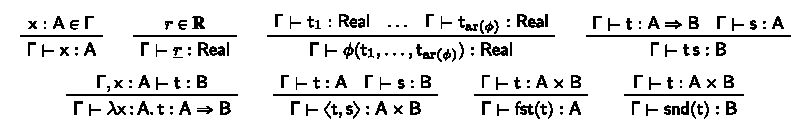
\includegraphics[width=0.95\linewidth,height=0.45\textheight,keepaspectratio]{typing-rules.pdf}\end{center}
 
Figure 1: Typing Rules.\par
 
% END S5.F1
 
% BEGIN S5.SS0.SSS0.P0.SPx1.p2
 
We denote the standard set theoretic interpretation of $\Lambda_{\mathsf{Real}}$ by $\llparenthesis-\rrparenthesis$. (See [25] for example.) To be concrete, the interpretation $\llparenthesis\mathsf{A}\rrparenthesis$ of a type $\mathsf{A}$ is a set inductively defined by\par
    \[\llparenthesis\mathsf{Real}\rrparenthesis=\mathbb{R},\qquad\llparenthesis%
\mathsf{A}\times\mathsf{B}\rrparenthesis=\llparenthesis\mathsf{A}%
\rrparenthesis\times\llparenthesis\mathsf{B}\rrparenthesis,\qquad%
\llparenthesis\mathsf{A}\Rightarrow\mathsf{B}\rrparenthesis=\llparenthesis%
\mathsf{A}\rrparenthesis\Rightarrow\llparenthesis\mathsf{B}\rrparenthesis;\]    
and we interpret a term $\mathsf{x}_{1}:\mathsf{A}_{1},\ldots,\mathsf{x}_{n}:\mathsf{A}_{n}\vdash%
\mathsf{t}:\mathsf{B}$ as a function $\llparenthesis\mathsf{t}\rrparenthesis$ from $\llparenthesis\mathsf{A}_{1}\rrparenthesis\times\cdots\times\llparenthesis%
\mathsf{A}_{n}\rrparenthesis$ to $\llparenthesis\mathsf{B}\rrparenthesis$. We give the definition of $\llparenthesis\mathsf{t}\rrparenthesis$ in Appendix C.\par
 
% END S5.SS0.SSS0.P0.SPx1.p2
 
% END S5.SS0.SSS0.P0.SPx1
 
% BEGIN S5.SS0.SSS0.P0.SPx2
 
\par\medskip\noindent\textbf{The Fundamental Lemma.}\par
 
% BEGIN S5.SS0.SSS0.P0.SPx2.p1
 
We inductively define a qq-metric space $\llbracket\mathsf{A}\rrbracket$ by\par
    \[\llbracket\mathsf{Real}\rrbracket=R,\qquad\llbracket\mathsf{A}\times\mathsf{B}%
\rrbracket=\llbracket\mathsf{A}\rrbracket\times\llbracket\mathsf{B}\rrbracket,%
\qquad\llbracket\mathsf{A}\Rightarrow\mathsf{B}\rrbracket=\llbracket\mathsf{A}%
\rrbracket\Rightarrow\llbracket\mathsf{B}\rrbracket.\]    
Here, $R$ is the qq-metric given in Example 10. Below, we simply denote the structure of an object $\llbracket\mathsf{A}\rrbracket$ by $(\mathcal{Q}_{\mathsf{A}},|\mathsf{A}|,\rho_{\mathsf{A}})$. It is straightforward to check that for every type $\mathsf{A}$, we have $|\mathsf{A}|=\llparenthesis\mathsf{A}\rrparenthesis$. The qq-metrics $\llbracket\mathsf{A}\rrbracket$ are the categorical interpretation of types $\mathsf{A}$, and the following fundamental lemma is derived from the categorical interpretation of $\Lambda_{\mathsf{Real}}$-terms in $\mathbf{Qqm}$.\par
 
% END S5.SS0.SSS0.P0.SPx2.p1
 
% BEGIN Thmtheorem11
 
\par\medskip\noindent\textbf{Theorem 11 (Fundamental Lemma).}\par
 
% BEGIN Thmtheorem11.p1
 
Let $\mathsf{\Gamma}=(\mathsf{x}_{1}:\mathsf{A}_{1},\ldots,\mathsf{x}_{n}:\mathsf{A%
}_{n})$ be a typing context. For every term $\mathsf{\Gamma}\vdash\mathsf{t}:\mathsf{A}$, and for every $(x,a,x^{\prime})\in\rho_{\mathsf{A}_{1}\times\cdots\times\mathsf{A}_{n}}$, we have\par
    \[(\llparenthesis\mathsf{t}\rrparenthesis\cdot x,\{\hskip-2.25pt|\mathsf{t}|%
\hskip-2.25pt\}\cdot x\cdot a,\llparenthesis\mathsf{t}\rrparenthesis\cdot x^{%
\prime})\in\rho_{{\mathsf{A}}}\]    
where we inductively define $\{\hskip-2.25pt|\mathsf{t}|\hskip-2.25pt\}\in\mathcal{Q}_{\mathsf{A}_{1}\times%
\cdots\times\mathsf{A}_{n}\Rightarrow\mathsf{B}}$ as follows:\par
  
\par\noindent  $\blacksquare$ 
% BEGIN S5.I1.i1.p1
 
We define $\{\hskip-2.25pt|\mathsf{x}_{i}|\hskip-2.25pt\}\cdot(x_{1},\ldots,x_{n})\cdot(a%
_{1},\ldots,a_{n})$ to be $a_{i}.$\par
 
% END S5.I1.i1.p1
 
 
\par\noindent  $\blacksquare$ 
% BEGIN S5.I1.i2.p1
 
We define $\{\hskip-2.25pt|\underline{r}|\hskip-2.25pt\}\cdot x\cdot a$ to be $\underline{0}.$\par
 
% END S5.I1.i2.p1
 
 
\par\noindent  $\blacksquare$ 
% BEGIN S5.I1.i3.p1
 
We define $\{\hskip-2.25pt|\phi(\mathsf{t}_{1},\ldots,\mathsf{t}_{n})|\hskip-2.25pt\}%
\cdot x\cdot a$ to be $\phi^{\mathrm{d}}(\llparenthesis\mathsf{t}_{1}\rrparenthesis\cdot x,\ldots,%
\llparenthesis\mathsf{t}_{n}\rrparenthesis\cdot x,\{\hskip-2.25pt|\mathsf{t}_{%
1}|\hskip-2.25pt\}\cdot x\cdot a,\ldots,\{\hskip-2.25pt|\mathsf{t}_{n}|\hskip-%
2.25pt\}\cdot x\cdot a)$ where we define $\phi^{\mathrm{d}}\colon\mathbb{R}^{n}\times[0,+\infty]^{n}\to[0,+\infty]$ by\par
    \[\phi^{\mathrm{d}}(y_{1},\ldots,y_{n},b_{1},\ldots,b_{n})=\bigwedge_{|y_{1}-z_{%
1}|\sqsupseteq b_{1}}\cdots\bigwedge_{|y_{n}-z_{n}|\sqsupseteq b_{n}}|\phi(y_{%
1},\ldots,y_{n})-\phi(z_{1},\ldots,z_{n})|.\]    
% END S5.I1.i3.p1
 
 
\par\noindent  $\blacksquare$ 
% BEGIN S5.I1.i4.p1
 
We define $\{\hskip-2.25pt|\mathsf{t}\,\mathsf{s}|\hskip-2.25pt\}\cdot x\cdot a$ to be $\{\hskip-2.25pt|\mathsf{t}|\hskip-2.25pt\}\cdot x\cdot a\cdot(\llparenthesis%
\mathsf{s}\rrparenthesis\cdot x)\cdot(\{\hskip-2.25pt|\mathsf{s}|\hskip-2.25pt%
\}\cdot x\cdot a)$.\par
 
% END S5.I1.i4.p1
 
 
\par\noindent  $\blacksquare$ 
% BEGIN S5.I1.i5.p1
 
We define $\{\hskip-2.25pt|\lambda\mathsf{x}\,{:}\,\mathsf{A}.\,\mathsf{t}|\hskip-2.25pt%
\}\cdot(x_{1},\ldots,x_{n})\cdot(a_{1},\ldots,a_{n})\cdot y\cdot b$ to be $\{\hskip-2.25pt|\mathsf{t}|\hskip-2.25pt\}\cdot(x_{1},\ldots,x_{n},y)\cdot(a_{%
1},\ldots,a_{n},b)$.\par
 
% END S5.I1.i5.p1
 
 
\par\noindent  $\blacksquare$ 
% BEGIN S5.I1.i6.p1
 
We define $\{\hskip-2.25pt|\langle\mathsf{t},\mathsf{s}\rangle|\hskip-2.25pt\}\cdot x\cdot
a$ to be $(\{\hskip-2.25pt|\mathsf{t}|\hskip-2.25pt\}\cdot x\cdot a,\{\hskip-2.25pt|%
\mathsf{s}|\hskip-2.25pt\}\cdot x\cdot a)$.\par
 
% END S5.I1.i6.p1
 
 
\par\noindent  $\blacksquare$ 
% BEGIN S5.I1.i7.p1
 
We define $\{\hskip-2.25pt|\mathsf{fst}(\mathsf{t})|\hskip-2.25pt\}\cdot x\cdot a$ to be the first component of $\{\hskip-2.25pt|\mathsf{t}|\hskip-2.25pt\}\cdot x\cdot a$.\par
 
% END S5.I1.i7.p1
 
 
\par\noindent  $\blacksquare$ 
% BEGIN S5.I1.i8.p1
 
We define $\{\hskip-2.25pt|\mathsf{snd}(\mathsf{t})|\hskip-2.25pt\}\cdot x\cdot a$ to be the second component of $\{\hskip-2.25pt|\mathsf{t}|\hskip-2.25pt\}\cdot x\cdot a$.\par
 
% END S5.I1.i8.p1
 
  
% END Thmtheorem11.p1
 
% END Thmtheorem11
 
% BEGIN S5.SS0.SSS0.P0.SPx2.p2
 
The fundamental lemma is a way to compositionally reason about distances.\par
 
% END S5.SS0.SSS0.P0.SPx2.p2
 
% BEGIN Thmtheorem12
 
\par\medskip\noindent\textbf{Example 12.}\par
 
% BEGIN Thmtheorem12.p1
 
Let us fix a positive real number $\epsilon$. We define $D_{\epsilon}\colon(\mathbb{R}\Rightarrow\mathbb{R})\to(\mathbb{R}\Rightarrow%
\mathbb{R})$ by\par
    \[D_{\epsilon}=\llparenthesis\lambda\mathsf{f}\,{:}\,\mathsf{Real}\Rightarrow%
\mathsf{Real}.\,\lambda\mathsf{x}\,{:}\,\mathsf{Real}.\,\mathrm{df}_{\epsilon}%
(f(\mathrm{ad}_{\epsilon}(\mathsf{x})),f(\mathsf{x}))\rrparenthesis\]    
where $\mathrm{df}_{\epsilon}(x,y)=\frac{x-y}{\epsilon}$ and $\mathrm{ad}_{\epsilon}(x)=x+\epsilon$. For $f\colon\mathbb{R}\to\mathbb{R}$ and $x\in\mathbb{R}$, $D_{\epsilon}\cdot f\cdot x$ calculates an approximation of the derivative of $f$ at $x$:\par
    \[D_{\epsilon}\cdot f\cdot x=\frac{f(x+\epsilon)-f(x)}{\epsilon}.\]    
By the fundamental lemma, we obtain $(D_{\epsilon},E_{\epsilon},D_{\epsilon})\in\rho_{(R\Rightarrow R)\Rightarrow(R%
\Rightarrow R)}$ where $E_{\epsilon}$ is a function from $|R\Rightarrow R|$ to $\mathcal{Q}_{R\Rightarrow R}\rightarrowtriangle\mathcal{Q}_{R\Rightarrow R}$ given by\par
    \[E_{\epsilon}\cdot f\cdot a=\lambda x:\mathbb{R}.\,\lambda b:[0,+\infty].\,%
\frac{a\cdot(x+\epsilon)\cdot b+a\cdot x\cdot b}{\epsilon}.\]    
We note that $E_{\epsilon}$ depends on our choice of term denoting $D_{\epsilon}$. In Example 15, we will observe that $(\mathrm{id}_{\mathbb{R}},a,\sin)$ is an element of $\rho_{R\Rightarrow R}$ where $\mathrm{id}_{\mathbb{R}}$ is the identity function on $\mathbb{R}$, and $a\in\mathcal{Q}_{R\Rightarrow R}$ is given by $a\cdot x\cdot b=|x-\sin(x)|+b$. By applying $(D_{\epsilon},E_{\epsilon},D_{\epsilon})$ to $(\mathrm{id}_{\mathbb{R}},a,\sin)$, we obtain $(D_{\epsilon}\cdot\mathrm{id}_{\mathbb{R}},a^{\prime},D_{\epsilon}\cdot\sin)%
\in\rho_{R}$ where\par
    \[a^{\prime}\cdot x\cdot b=\frac{|x+\epsilon-\sin(x+\epsilon)|+|x-\sin(x)|+2b}{%
\epsilon}.\]    
From this, we see that the distance between $D_{\epsilon}\cdot\mathrm{id}_{\mathbb{R}}\cdot 0$ and $D_{\epsilon}\cdot{\sin}\cdot 0$ is bounded by $\frac{|\epsilon-\sin(\epsilon)|}{\epsilon}$. We note that $a^{\prime}$ is not the exact distance between $D_{\epsilon}\cdot\mathrm{id}_{\mathbb{R}}$ and $D_{\epsilon}\cdot\sin$. For example, while $|D_{0.1}\cdot\mathrm{id}_{\mathbb{R}}\cdot 0-D_{0.1}\cdot{\sin}\cdot 0.1|%
\approx 0.01$, we have $a^{\prime}\cdot 0\cdot 0.1\approx 2$. This gap stems in the fact that $(D_{\epsilon},E_{\epsilon},D_{\epsilon})$ takes all functions into account and cannot exploit continuity of specific functions.\par
 
% END Thmtheorem12.p1
 
% END Thmtheorem12
 
% END S5.SS0.SSS0.P0.SPx2
 
% END S5


% BEGIN S6
 
\par\medskip\noindent\textbf{6 Quasi-Metric Logical Relations}\par
 
% BEGIN S6.p1
 
As described in Section 3, any qq-metric gives rise to left and right observational quasi-metrics. In this section, we introduce a class of logical relations $\gamma_{\mathsf{A}}$ that capture the left observational quasi-metric associated to $\rho_{{\mathsf{A}}}$. We will then show how such relations can be used to derive over-approximations of distances between functions.\par
 
% END S6.p1
 
% BEGIN S6.p2
 
For a type $\mathsf{A}$, we define $\gamma_{\mathsf{A}}\subseteq|\mathsf{A}|\times\mathcal{Q}_{\mathsf{A}}\times|%
\mathsf{A}|$ by induction on $\mathsf{A}$ as follows:\par
    $\displaystyle(x,a,x^{\prime})\in\gamma_{\mathsf{Real}}$ $\displaystyle\iff|x-x^{\prime}|\sqsupseteq a,$     $\displaystyle(f,a,f^{\prime})\in\gamma_{\mathsf{A}\Rightarrow\mathsf{B}}$ $\displaystyle\iff\text{for all }(x,b,x^{\prime})\in\rho_{\mathsf{A}},\,(f\cdot
x%
,a\cdot x\cdot b,f^{\prime}\cdot x)\in\gamma_{\mathsf{B}},\text{ and}$      $\displaystyle\mathrel{\phantom{\iff}}\text{for all }(f^{\prime},b,f^{\prime})%
\in\rho_{\mathsf{A}\Rightarrow\mathsf{B}},\,(f,a\otimes b,f)\in\rho_{\mathsf{A%
}\Rightarrow\mathsf{B}},$     $\displaystyle((x,y),(a,b),(x^{\prime},y^{\prime}))\in\gamma_{\mathsf{A}\times%
\mathsf{B}}$ $\displaystyle\iff(x,a,x^{\prime})\in\gamma_{\mathsf{A}}\text{ and }(y,b,y^{%
\prime})\in\gamma_{\mathsf{B}}.$    
We give some explanation on the definition of $\gamma_{\mathsf{A}\Rightarrow\mathsf{B}}$. The definition consists of two conditions. The first condition means that, if $(f,a,f^{\prime})$ is an element of $\gamma_{\mathsf{A}\Rightarrow\mathsf{B}}$, then the distance $a\cdot x\cdot b$ over-approximates the distance between $f$ and $f^{\prime}$ at the same point $x$ (rather than on distinct points, as is the case for the relation $\rho_{\mathsf{A}\Rightarrow\mathsf{B}}$). The second condition means that $a$ also over-approximates the gap between the self-distance of $f^{\prime}$ and the self-distance of $f$.\par
 
% END S6.p2
 
% BEGIN S6.p3
 
Recall that $\rho_{\mathsf{A}}^{l}$ is the quasi-metric representing the left observational quasi-metrics associated with the qq-metric $\rho_{\mathsf{A}}$. In Appendix D, we give some auxiliary lemmas and proofs for Proposition 13 and Theorem 14.\par
 
% END S6.p3

% BEGIN S6.p4
 
We can use Proposition 13 to over-approximate $\rho$-distances in terms of $\gamma$-distances and the left observational quasi-metric. Let us sketch our idea. First, thanks to Proposition 13 and Proposition 6, we can exploit left-transitivity to pass from a $\gamma$-distance between $\mathsf{t}$ and $\mathsf{s}$ and a self-$\rho$-distance of $\mathsf{s}$ to a $\rho$-distance between $\mathsf{t}$ and $\mathsf{s}$:\par
    $\displaystyle(\llparenthesis\mathsf{t}\rrparenthesis,a,\llparenthesis\mathsf{s%
}\rrparenthesis)\in\gamma_{\mathsf{A}}\ \text{and}\ (\llparenthesis\mathsf{s}%
\rrparenthesis,b,\llparenthesis\mathsf{s}\rrparenthesis)\in\rho_{{\mathsf{A}}}%
\ \implies\ (\llparenthesis\mathsf{t}\rrparenthesis,a\otimes b,\llparenthesis%
\mathsf{s}\rrparenthesis)\in\rho_{{\mathsf{A}}}.$  (left transitivity)   
Second, thanks to the fundamental lemma, we can always obtain a $\rho$-distance by summing a $\gamma$-distance with the self-distance $\{\hskip-2.25pt|\mathsf{s}|\hskip-2.25pt\}$:\par
    $\displaystyle(\llparenthesis\mathsf{t}\rrparenthesis,a,\llparenthesis\mathsf{s%
}\rrparenthesis)\in\gamma_{\mathsf{A}}\ \implies\ (\llparenthesis\mathsf{t}%
\rrparenthesis,a\otimes\{\hskip-2.25pt|\mathsf{s}|\hskip-2.25pt\},%
\llparenthesis\mathsf{s}\rrparenthesis)\in\rho_{{\mathsf{A}}}.$  ($\rho\sqsupseteq\gamma\ \otimes$ self-$\rho$)   
The following result exploits this last idea to bound the distance between two functions $f$ and $g$ by summing the “vertical distance” between $f$ and $g$ (that is, the distance of $f(x)$ and $g(x)$ for some fixed $x$) with an approximation of the self-distances of $f$ and $g$:\par
 
% END S6.p4

% BEGIN Thmtheorem15
 
\par\medskip\noindent\textbf{Example 15.}\par
 
% BEGIN Thmtheorem15.p1
 
Let $\mathrm{id}_{\mathbb{R}}$ be the identity function on $\mathbb{R}$. By the fundamental lemma with a simple calculation, we obtain $(\mathrm{id}_{\mathbb{R}},a^{\prime},\mathrm{id}_{\mathbb{R}})\in\rho_{R%
\Rightarrow R}$ and $(\sin,a^{\prime},\sin)\in\rho_{R\Rightarrow R}$ where $a^{\prime}\cdot x\cdot b=b$. By Theorem 14, $a\in\mathcal{Q}_{R\Rightarrow R}$ given by $a\cdot x\cdot b=|x-\sin(x)|$ satisfies $(\mathrm{id}_{\mathbb{R}},a\otimes a^{\prime},\sin)\in\rho_{R\Rightarrow R}$. To be concrete, $(a\otimes a^{\prime})\cdot x\cdot b=|x-\sin(x)|+b$, which means that the distance between $x$ and $\sin(y)$ is small when $x$ and $y$ are close to $0$.\par
 
% END Thmtheorem15.p1
 
% END Thmtheorem15
 
% BEGIN Thmtheorem16
 
\par\medskip\noindent\textbf{$\blacktriangleright$ Remark 16.}\par
 
% BEGIN Thmtheorem16.p1
 
Due to asymmetry in the definition of the exponential $X\Rightarrow Y$ in $\mathbf{Qqm}$, it is not clear how to capture the right observational quasi-metrics in a similar manner. However, we will see that right observational quasi-metrics can be captured by partial metric logical relations introduced in the next section.\par
 
% END Thmtheorem16.p1
 
% END Thmtheorem16
 
% END S6


% BEGIN S7
 
\par\medskip\noindent\textbf{7 Partial Metric Logical Relations}\par
 
% BEGIN S7.p1
 
As discussed in Section 3, the qq-metrics $\rho_{\mathsf{A}}$ are not, in general, partial metrics. In this section we introduce a family of differential logical relations $(\eta_{\mathsf{A}})_{\mathsf{A}\in\mathsf{Types}}$ that defines a class of partial quasi-metrics over $\Lambda_{\mathsf{Real}}$. The fundamental (indeed, the only) difference with respect to the family $\rho_{\mathsf{A}}$ is, as it may be expected, in the case of the function type.\par
 
% END S7.p1
 
% BEGIN S7.p2
 
For any type $\mathsf{A}$, we define $\eta_{\mathsf{A}}\subseteq|\mathsf{A}|\times\mathcal{Q}_{\mathsf{A}}\times|%
\mathsf{A}|$ by induction on $\mathsf{A}$ as follows:\par
    $\displaystyle(x,a,x^{\prime})\in\eta_{\mathsf{Real}}$ $\displaystyle\iff|x-x^{\prime}|\sqsupseteq a,$     $\displaystyle(f,a,f^{\prime})\in\eta_{\mathsf{A}\Rightarrow\mathsf{B}}$ $\displaystyle\iff\text{there are }a_{1},a_{2}\in\mathcal{Q}_{\mathsf{A}%
\Rightarrow\mathsf{B}}\text{ such that }a_{1}\otimes a_{2}\sqsupseteq a\text{ %
and }$      $\displaystyle\phantom{{}\iff{}}\text{for all }(x,b,x^{\prime})\in\eta_{\mathsf%
{A}},\ (f\cdot x,a_{1}\cdot x\cdot b,f\cdot x^{\prime})\in\eta_{\mathsf{B}}%
\text{ and }$      $\displaystyle\phantom{{}\iff{}\text{for all }(x,b,x^{\prime})\in\eta_{\mathsf{%
A}}\ }(f\cdot x^{\prime},a_{2}\cdot x\cdot b,f^{\prime}\cdot x^{\prime})\in%
\eta_{\mathsf{B}},$     $\displaystyle((x,y),(a,b),(x^{\prime},y^{\prime}))\in\eta_{\mathsf{A}\times%
\mathsf{B}}$ $\displaystyle\iff(x,a,x^{\prime})\in\eta_{\mathsf{A}}\text{ and }(y,b,y^{%
\prime})\in\eta_{\mathsf{B}}.$    
The idea of the definition of $\eta_{\mathsf{A}\Rightarrow\mathsf{B}}$ is that if $(f,a,f^{\prime})\in\eta_{\mathsf{A}\Rightarrow\mathsf{B}}$, then $a$ must be larger than or equal to the sum of the self-distance of $f$ and of the “vertical” distances between $f$ and $f^{\prime}$. The following result shows that the relations $\eta_{\mathsf{A}}$ define partial quasi-metrics on all types.\par
 
% END S7.p2
 
% BEGIN S7.p3
 
For $(f,a,f^{\prime})\in\eta_{\mathsf{A}\Rightarrow\mathsf{B}}$, we call a pair $a_{1},a_{2}\in\mathcal{Q}_{\mathsf{A}\Rightarrow\mathsf{B}}$ satisfying the condition in the definition of $(f,a,f^{\prime})\in\eta_{\mathsf{A}\Rightarrow\mathsf{B}}$ a decomposition of $(f,a,f^{\prime})\in\eta_{\mathsf{A}\Rightarrow\mathsf{B}}$.\par
 
% END S7.p3
 
% BEGIN Thmtheorem17
 
\par\medskip\noindent\textbf{Proposition 17.}\par
 
% BEGIN Thmtheorem17.p1
 
For all types $\mathsf{A}$:\par
  
\par\noindent  $\blacksquare$ 
% BEGIN S7.I1.i1.p1
 
For any type $\mathsf{A}$, the relation $\rho_{\mathsf{A}}$ is $\mathcal{Q}$-closed. In particular, for all $(x,a,x^{\prime})\in\eta_{\mathsf{A}}$, the set of decompositions of $(x,a,x^{\prime})\in\eta_{\mathsf{A}}$ is a complete lattice.\par
 
% END S7.I1.i1.p1
 
 
\par\noindent  $\blacksquare$ 
% BEGIN S7.I1.i2.p1
 
If $(x,a,x^{\prime})\in\eta_{\mathsf{A}}$, then $(x,a,x)\in\eta_{\mathsf{A}}$.\par
 
% END S7.I1.i2.p1
 
 
\par\noindent  $\blacksquare$ 
% BEGIN S7.I1.i3.p1
 
If $(x,a,z)\in\eta_{\mathsf{A}}$ and $(z,b,y)\in\eta_{\mathsf{A}}$, then there exists $c_{1},c_{2}\in\mathcal{Q}_{\mathsf{A}}$ such that $a\otimes b\sqsubseteq c_{1}\otimes c_{2}$, $(z,c_{1},z)\in\eta_{\mathsf{A}}$ and $(x,c_{2},y)\in\eta_{\mathsf{A}}$. In particular, $(x,a\otimes(c_{1}\multimap b),y)\in\eta_{\mathsf{A}}$.\par
 
% END S7.I1.i3.p1
 
  
% END Thmtheorem17.p1
 
% END Thmtheorem17
 
% BEGIN S7.p4
 
By adapting the definition of $\gamma_{\mathsf{A}}$ from Section 6, we can capture the left observational quasi-metrics $\rho_{\mathsf{A}}^{l}$ associated with the partial quasi-metrics $\eta_{\mathsf{A}}$. Moreover, by Proposition 8, the right observational quasi-metric $\rho_{\mathsf{A}}^{r}$ satisfies $(x,\widehat{\eta}_{\mathsf{A}}(x,x)\multimap a,y)\in\rho_{\mathsf{A}}^{r}\ %
\iff(x,a,y)\in\eta_{\mathsf{A}}$. Thanks to this, we can capture this quasi-metrics via the logical relations $\delta_{\mathsf{A}}\subseteq|\mathsf{A}|\times\mathcal{Q}_{\mathsf{A}}\times|%
\mathsf{A}|$ defined by induction on $\mathsf{A}$, letting the base and product case being defined as for $\gamma_{\mathsf{A}}$, and the function case being as follows:\par
    $\displaystyle(f,a,f^{\prime})\in\delta_{\mathsf{A}\Rightarrow\mathsf{B}}$ $\displaystyle\iff\text{for all }(f,b,f)\in\eta_{\mathsf{A}\Rightarrow\mathsf{B%
}},\ (f,a\otimes b,f^{\prime})\in\eta_{\mathsf{A}\Rightarrow\mathsf{B}}.$    
% END S7.p4

% BEGIN Thmtheorem13
 
\par\medskip\noindent\textbf{Proposition 13.}\par
 
% BEGIN Thmtheorem13.p1
 
For every type $\mathsf{A}$, we have $\rho^{l}_{{\mathsf{A}}}=\gamma_{\mathsf{A}}$.\par
 
% END Thmtheorem13.p1
 
% END Thmtheorem13

% BEGIN Thmtheorem14
 
\par\medskip\noindent\textbf{Theorem 14.}\par
 
% BEGIN Thmtheorem14.p1
 
Let $\mathsf{A}$ be a type. For any $f,f^{\prime}\in|\mathsf{A}\Rightarrow\mathsf{Real}|$ and any $a,a^{\prime}\in\mathcal{Q}_{\mathsf{A}\Rightarrow\mathsf{Real}}$, if\par
  
\par\noindent  $\blacksquare$ 
% BEGIN S6.I1.i1.p1
 
$|f\cdot x-f^{\prime}\cdot x|\sqsupseteq a\cdot x\cdot b$ for all $(x,b,x^{\prime})\in\rho_{\mathsf{A}}$; and\par
 
% END S6.I1.i1.p1
 
 
\par\noindent  $\blacksquare$ 
% BEGIN S6.I1.i2.p1
 
$(f,a^{\prime},f)\in\rho_{\mathsf{A}\Rightarrow\mathsf{Real}}$ and $(f^{\prime},a^{\prime},f^{\prime})\in\rho_{\mathsf{A}\Rightarrow\mathsf{Real}}$,\par
 
% END S6.I1.i2.p1
 
  
then $(f,a\otimes a^{\prime},f^{\prime})\in\rho_{\mathsf{A}\Rightarrow\mathsf{Real}}$.\par
 
% END Thmtheorem14.p1
 
% END Thmtheorem14

% BEGIN Thmtheorem18
 
\par\medskip\noindent\textbf{Proposition 18.}\par
 
% BEGIN Thmtheorem18.p1
 
For every type $\mathsf{A}$, we have $\rho_{\mathsf{A}}^{r}=\delta_{\mathsf{A}}$.\par
 
% END Thmtheorem18.p1
 
% END Thmtheorem18

% BEGIN A1
 
\par\medskip\noindent\textbf{Appendix A Proofs for Section 3}\par
 
% BEGIN A1.SS0.SSS0.P0.SPx1
 
\par\medskip\noindent\textbf{Proof of Proposition 7.}\par
 
% BEGIN A1.SS0.SSS0.P0.SPx1.p1
 
Suppose there exists a quasi-metric $q\sqsupseteq s$ such that $s\otimes q\sqsubseteq s$ holds. Then $s\otimes s\sqsubseteq s\otimes q\sqsubseteq s$, so $s$ is transitive. A similar argument works if $q$ is such that $q\otimes s\sqsubseteq s$. Conversely, if $s$ is a qq-metric it is enough to let $q:=s^{r}$ and use Proposition 6 (iv). $\hfill\blacktriangleleft$\par
 
% END A1.SS0.SSS0.P0.SPx1.p1
 
% END A1.SS0.SSS0.P0.SPx1
 
% BEGIN A1.SS0.SSS0.P0.SPx2
 
\par\medskip\noindent\textbf{Proof of Proposition 8.}\par
 
% BEGIN A1.SS0.SSS0.P0.SPx2.p1
 
We only argue for $c=r$, the other case being similar. From $s^{r}(x,y)=\bigwedge_{z}s(z,x)\multimap s(z,y)\sqsubseteq s(x,x)\multimap s(x,%
y)=(\Theta^{r}_{s})(x,y)$ we deduce that $s^{r}\sqsubseteq\Theta^{r}_{s}$. The converse direction $s^{r}\sqsupseteq\Theta^{r}_{s}$ corresponds to showing that $s(z,x)\otimes(s(x,x)\multimap s(x,y))\sqsubseteq s(z,y)$, which holds iff $s$ is a partial quasi-metric. We have thus shown that $s$ is a PQM iff $\Theta^{r}_{s}=s^{r}$. This also implies that, if $s$ is a PWM, $\Theta^{r}_{s}$ is a quasi-metric. Finally, suppose $\Theta^{r}_{s}$ is a quasi-metric. By quasi-reflexivity, and the divisibility of $\mathcal{Q}$, we have that $s(x,z)=s(x,x)\otimes(s(x,x)\multimap s(x,z))$. We then have $s(x,z)\otimes(s(z,z)\multimap s(z,y))=s(x,x)\otimes(s(x,x)\multimap s(x,z))%
\otimes(s(z,z)\multimap s(z,y))\sqsubseteq s(x,y)$, so $s$ is a partial quasi-metric. $\hfill\blacktriangleleft$\par
 
% END A1.SS0.SSS0.P0.SPx2.p1
 
% BEGIN Thmtheorem21
 
\par\medskip\noindent\textbf{Lemma 21.}\par
 
% BEGIN Thmtheorem21.p1
 
The map $\rho\mapsto\widehat{\rho}$ defines a bijection between the $\mathcal{Q}$-closed relations $\rho\subseteq X\times\mathcal{Q}\times X$ and $\mathcal{Q}\mathbf{Rel}(X,X)$.\par
 
% END Thmtheorem21.p1
 
% END Thmtheorem21
 
% END A1.SS0.SSS0.P0.SPx2
 
% BEGIN A1.SS0.SSS0.P0.SPx3
 
\par\medskip\noindent\textbf{Proof.}\par
 
% BEGIN A1.SS0.SSS0.P0.SPx3.p1
 
Let $\rho,\tau$ be closed and let $\widehat{\rho}(x,y)=\widehat{\tau}(x,y)$. Observe that, for all $x,y\in X$, by $\mathcal{Q}$-closure we have $(x,\widehat{\rho}(x,y),y)\in\rho$. Suppose now that $(x,a,y)\in\tau$, then $a\sqsubseteq\widehat{\tau}(x,y)=\widehat{\rho}(x,y)$, and from $(x,\widehat{\rho}(x,y),y)\in\rho$ and $a\sqsubseteq\widehat{\rho}(x,y)$ we deduce $(x,a,y)\in\rho$. By a similar argument we can also prove that $(x,a,y)\in\rho$ implies $(x,a,y)\in\tau$, so in the end $\rho=\tau$. We conclude then that the map $\rho\mapsto\widehat{\rho}$ is injective. For surjectivity, observe that any $s\in\mathcal{Q}\mathbf{Rel}(X,X)$ induces a relation $(x,a,y)\in\rho^{s}$ iff $a\sqsubseteq s(x,y)$, so that $s=\widehat{\rho^{s}}$. $\hfill\blacktriangleleft$\par
 
% END A1.SS0.SSS0.P0.SPx3.p1
 
% END A1.SS0.SSS0.P0.SPx3
 
% END A1


% BEGIN A2
 
\par\medskip\noindent\textbf{Appendix B Details of Cartesian Closed Structure}\par
 
% BEGIN A2.p1
 
The first projection from $X\times Y$ to $Y$ is given by $(\mathrm{proj}_{X,Y},\varpi_{X,Y},\mathrm{proj}_{X,Y})$ consisting of the first projection $\mathrm{proj}_{X,Y}\colon|X|\times|Y|\to|X|$ and $\varpi_{X,Y}\colon|X|\times|Y|\to(\mathcal{Q}_{X}\times\mathcal{Q}_{Y}%
\rightarrowtriangle\mathcal{Q}_{X})$ given by $\varpi_{X,Y}\cdot(x,y)\cdot(a,b)=a$. The second projection is given in the same manner. The tupling of $(f,a,f^{\prime})\colon Z\to X$ and $(g,b,g^{\prime})\colon Z\to Y$ is $(\langle f,g\rangle,\langle a,b\rangle,\langle f^{\prime},g^{\prime}\rangle)$ where $\langle f,g\rangle\colon|Z|\to|X|\times|Y|$ and $\langle a,b\rangle\colon|Z|\to(\mathcal{Q}_{Z}\rightarrowtriangle\mathcal{Q}_{%
X}\times\mathcal{Q}_{Y})$ are the tupling of $f,g$ and $a,b$ respectively, that is, $\langle f,g\rangle\cdot z$ is defined to be $(f\cdot z,g\cdot z)$, and $\langle a,b\rangle\cdot z\cdot c$ is defined to be $(a\cdot z\cdot c,a\cdot z\cdot c)$. The currying of $(f,a,f^{\prime})\colon Z\times X\to Y$ is $(f^{\wedge},a^{\wedge},f^{\prime\wedge})$ where $f^{\wedge}\colon|Z|\to(|X|\Rightarrow|Y|)$ and $f^{\prime\wedge}\colon|Z|\to(|X|\Rightarrow|Y|)$ are the currying of $f\colon|Z|\times|X|\to|Y|$ and $f^{\prime}\colon|Z|\times|X|\to|Y|$, and $a^{\wedge}\colon|Z|\to(\mathcal{Q}_{Z}\rightarrowtriangle\mathcal{Q}_{X%
\Rightarrow Y})$ is the currying of $a\colon|Z|\times|X|\to(\mathcal{Q}_{Z\times X}\rightarrowtriangle\mathcal{Q}_{%
Y}),$ namely, $a^{\wedge}\cdot z\cdot a\cdot x\cdot b$ is defined to be $a\cdot(z,x)\cdot(a,b)$. The evaluation morphism $(\mathrm{eval}_{X,Y},\varepsilon_{X,Y},\mathrm{eval}_{X,Y})\colon(X\Rightarrow
Y%
)\times X\to Y$ consists of the evaluation function $\mathrm{eval}_{X,Y}\colon(|X|\Rightarrow|Y|)\times|X|\to|Y|$ and $\varepsilon_{X,Y}$ is given by $\varepsilon_{X,Y}\cdot(a,b)\cdot(f,x)=a\cdot x\cdot b.$\par
 
% END A2.p1
 
% END A2


% BEGIN A3
 
\par\medskip\noindent\textbf{Appendix C Definitions and Proofs for Section 5}\par
 
% BEGIN A3.p1
 
In Figure 4, we define the function $\llparenthesis\mathsf{t}\rrparenthesis$ by induction on the type derivation of $t$.\par
 
% END A3.p1
 
% BEGIN A3.F4
    $\displaystyle\llparenthesis\mathsf{x}_{i}\rrparenthesis\cdot(x_{1},\ldots,x_{n})$ $\displaystyle=x_{i},$     $\displaystyle\llparenthesis\underline{r}\rrparenthesis\cdot(x_{1},\ldots,x_{n})$ $\displaystyle=r,$     $\displaystyle\llparenthesis\phi(\mathsf{t}_{1},\ldots,\mathsf{t}_{\mathrm{ar}(%
\phi)})\rrparenthesis\cdot(x_{1},\ldots,x_{n})$ $\displaystyle=\phi(\llparenthesis\mathsf{t}_{1}\rrparenthesis\cdot(x_{1},%
\ldots,x_{n}),\ldots,\llparenthesis\mathsf{t}_{\mathrm{ar}(\phi)}%
\rrparenthesis\cdot(x_{1},\ldots,x_{n})),$     $\displaystyle\llparenthesis\mathsf{t}\,\mathsf{s}\rrparenthesis\cdot(x_{1},%
\ldots,x_{n})$ $\displaystyle=\llparenthesis\mathsf{t}\rrparenthesis\cdot(x_{1},\ldots,x_{n})%
\cdot(\llparenthesis\mathsf{s}\rrparenthesis\cdot(x_{1},\ldots,x_{n})),$     $\displaystyle\llparenthesis\lambda\mathsf{x}\,{:}\,\mathsf{A}.\,\mathsf{t}%
\rrparenthesis\cdot(x_{1},\ldots,x_{n})\cdot y$ $\displaystyle=\llparenthesis\mathsf{t}\rrparenthesis\cdot(x_{1},\ldots,x_{n},y),$     $\displaystyle\llparenthesis\mathsf{fst}(\mathsf{t})\rrparenthesis\cdot(x_{1},%
\ldots,x_{n})$ $\displaystyle=\text{the first component of }\llparenthesis\mathsf{t}%
\rrparenthesis\cdot(x_{1},\ldots,x_{n}),$     $\displaystyle\llparenthesis\mathsf{snd}(\mathsf{t})\rrparenthesis\cdot(x_{1},%
\ldots,x_{n})$ $\displaystyle=\text{the second component of }\llparenthesis\mathsf{t}%
\rrparenthesis\cdot(x_{1},\ldots,x_{n}),$     $\displaystyle\llparenthesis\langle\mathsf{t},\mathsf{s}\rangle\rrparenthesis%
\cdot(x_{1},\ldots,x_{n})$ $\displaystyle=(\llparenthesis\mathsf{t}\rrparenthesis\cdot(x_{1},\ldots,x_{n})%
,\llparenthesis\mathsf{s}\rrparenthesis\cdot(x_{1},\ldots,x_{n})).$    
Figure 4: Set Theoretic Denotation of Terms.\par
 
% END A3.F4
 
% BEGIN A3.SS0.SSS0.P0.SPx1
 
\par\medskip\noindent\textbf{Proof of Theorem 11.}\par
 
% BEGIN A3.SS0.SSS0.P0.SPx1.p1
 
The triple $(\llparenthesis\mathsf{t}\rrparenthesis,\{\hskip-2.25pt|\mathsf{t}|\hskip-2.25%
pt\},\llparenthesis\mathsf{t}\rrparenthesis)$ is the interpretation of $\mathsf{\Gamma}\vdash\mathsf{t}:\mathsf{A}$ in the cartesian closed category $\mathbf{Qqm}$ where we interpret $\mathsf{\Gamma}\vdash\phi(\mathsf{t}_{1},\ldots,\mathsf{t}_{n})$ by\par
    \[\llbracket\mathsf{A}_{1}\rrbracket\times\cdots\times\llbracket\mathsf{A}_{n}%
\rrbracket\xrightarrow{\langle\llbracket\mathsf{t}_{1}\rrbracket,\ldots,%
\llbracket\mathsf{t}_{n}\rrbracket\rangle}R\times\cdots\times R\xrightarrow{(%
\phi,\phi^{\mathrm{d}},\phi)}R.\]    
The statement follows from that $(\llparenthesis\mathsf{t}\rrparenthesis,\{\hskip-2.25pt|\mathsf{t}|\hskip-2.25%
pt\},\llparenthesis\mathsf{t}\rrparenthesis)$ is a morphism from $\llbracket\mathsf{A}_{1}\rrbracket\times\cdots\times\llbracket\mathsf{A}_{n}\rrbracket$ to $\llbracket\mathsf{A}\rrbracket$ in $\mathbf{Qqm}$. $\hfill\blacktriangleleft$\par
 
% END A3.SS0.SSS0.P0.SPx1.p1
 
% END A3.SS0.SSS0.P0.SPx1
 
% END A3


% BEGIN A4
 
\par\medskip\noindent\textbf{Appendix D Proofs for Section 6}\par
 
% BEGIN A4.p1
 
Let us introduce a notation. For a type $\mathsf{A}$ and $x\in|\mathsf{A}|$, we write $\lceil x\rceil\in\mathcal{Q}_{\mathsf{A}}$ for $\widehat{\rho_{\mathsf{A}}}(x,x)$, i.e., $\lceil x\rceil$ is equal to $\sup\{a\in\mathcal{Q}_{\mathsf{A}}\mid(x,a,x)\in\rho_{\mathsf{A}}\}.$ Since $\rho_{\mathsf{A}}$ is closed under supremum, for any $x\in|\mathsf{A}|$, we have $(x,\lceil x\rceil,x)\in\rho_{\mathsf{A}}$.\par
 
% END A4.p1
 
% BEGIN Thmtheorem22
 
\par\medskip\noindent\textbf{Lemma 22.}\par
 
% BEGIN Thmtheorem22.p1
 
For every type $\mathsf{A}$ and for every $x,x^{\prime}\in|\mathsf{A}|$, if $(x,\lceil x\rceil,x^{\prime})\in\rho_{\mathsf{A}}$, then $x=x^{\prime}$.\par
 
% END Thmtheorem22.p1
 
% END Thmtheorem22
 
% BEGIN A4.SS0.SSS0.P0.SPx1
 
\par\medskip\noindent\textbf{Proof.}\par
 
% BEGIN A4.SS0.SSS0.P0.SPx1.p1
 
By induction on $\mathsf{A}$. It is straightforward to check the case $\mathsf{Real}$ and the case $\mathsf{A}\times\mathsf{B}$. For the case $\mathsf{A}\Rightarrow\mathsf{B}$, if $(f,\lceil f\rceil,f^{\prime})\in\rho_{\mathsf{A}\Rightarrow\mathsf{B}}$, then for any $x\in|\mathsf{A}|$, we have\par
    \[(f\cdot x,\lceil f\rceil\cdot x\cdot\lceil x\rceil,f^{\prime}\cdot x)\in\rho_{%
\mathsf{A}}.\]    
Here, by the induction hypothesis,\par
    $\displaystyle\lceil f\rceil\cdot x\cdot\lceil x\rceil$ $\displaystyle=\sup\{a\in\mathcal{Q}_{\mathsf{B}}\mid\text{for all }(x,\lceil x%
\rceil,x^{\prime})\in\rho_{\mathsf{A}},\,(f\cdot x,a,f\cdot x^{\prime})\in\rho%
_{\mathsf{B}}\}$      $\displaystyle=\sup\{a\in\mathcal{Q}_{\mathsf{B}}\mid(f\cdot x,a,f\cdot x)\in%
\rho_{\mathsf{B}}\}=\lceil f\cdot x\rceil.$    
Hence, $f^{\prime}\cdot x=f\cdot x$. $\hfill\blacktriangleleft$\par
 
% END A4.SS0.SSS0.P0.SPx1.p1
 
% BEGIN Thmtheorem23
 
\par\medskip\noindent\textbf{Lemma 23.}\par
 
% BEGIN Thmtheorem23.p1
 
For any type $\mathsf{A}$ and $\mathsf{B}$, if $f\in|\mathsf{A}\Rightarrow\mathsf{B}|$ and $x\in|\mathsf{A}|$, then $\lceil f\rceil\cdot x\cdot\lceil x\rceil=\lceil f\cdot x\rceil$.\par
 
% END Thmtheorem23.p1
 
% END Thmtheorem23
 
% END A4.SS0.SSS0.P0.SPx1
 
% BEGIN A4.SS0.SSS0.P0.SPx2
 
\par\medskip\noindent\textbf{Proof.}\par
 
% BEGIN A4.SS0.SSS0.P0.SPx2.p1
 
This is shown in the proof of Lemma 22. $\hfill\blacktriangleleft$\par
 
% END A4.SS0.SSS0.P0.SPx2.p1
 
% BEGIN Thmtheorem24
 
\par\medskip\noindent\textbf{Lemma 24.}\par
 
% BEGIN Thmtheorem24.p1
 
For every type $\mathsf{A}$, if $(x,a\otimes\lceil x^{\prime}\rceil,x^{\prime})\in\rho_{\mathsf{A}}$, then $(x,a,x^{\prime})\in\gamma_{\mathsf{A}}$.\par
 
% END Thmtheorem24.p1
 
% END Thmtheorem24
 
% END A4.SS0.SSS0.P0.SPx2
 
% BEGIN A4.SS0.SSS0.P0.SPx3
 
\par\medskip\noindent\textbf{Proof.}\par
 
% BEGIN A4.SS0.SSS0.P0.SPx3.p1
 
By induction on $\mathsf{A}$. The only non-trivial case is $\mathsf{A}\Rightarrow\mathsf{B}$. If $(f,a\otimes\lceil f^{\prime}\rceil,f^{\prime})\in\rho_{\mathsf{A}\Rightarrow%
\mathsf{B}}$, then for any $(x,b,x^{\prime})\in\rho_{\mathsf{A}}$, since $(x,b\vee\lceil x\rceil,x)\in\rho_{\mathsf{A}}$, we obtain\par
    \[(f\cdot x,(a\cdot x\cdot(b\vee\lceil x\rceil))\otimes(\lceil f^{\prime}\rceil%
\cdot x\cdot(b\vee\lceil x\rceil)),f^{\prime}\cdot x)\in\rho_{\mathsf{B}}.\]    
It follows from monotonicity of $a$ and Lemma 23 that we have\par
    \[(f\cdot x,(a\cdot x\cdot b)\otimes(\lceil f^{\prime}\rceil\cdot x\cdot\lceil x%
\rceil),f^{\prime}\cdot x)=(f\cdot x,(a\cdot x\cdot b)\otimes\lceil f^{\prime}%
\cdot x\rceil,f^{\prime}\cdot x)\in\rho_{\mathsf{B}}.\]    
By the induction hypothesis, we conclude $(f\cdot x,a\cdot x\cdot b,f^{\prime}\cdot x)\in\gamma_{\mathsf{B}}$. For any $(f^{\prime},b,f^{\prime})\in\rho_{\mathsf{A}\Rightarrow\mathsf{B}}$, since $b\sqsubseteq\lceil f^{\prime}\rceil$, it follows from $(f,a\otimes\lceil f^{\prime}\rceil,f^{\prime})\in\rho_{\mathsf{A}\Rightarrow%
\mathsf{B}}$ that $(f,a\otimes b,f^{\prime})\in\rho_{\mathsf{A}\Rightarrow\mathsf{B}}$. By left-quasi-reflexivity, we obtain $(f,a\otimes b,f)\in\rho_{\mathsf{A}\Rightarrow\mathsf{B}}$. $\hfill\blacktriangleleft$\par
 
% END A4.SS0.SSS0.P0.SPx3.p1
 
% END A4.SS0.SSS0.P0.SPx3
 
% BEGIN A4.SS0.SSS0.P0.SPx4
 
\par\medskip\noindent\textbf{Proof of Proposition 13.}\par
 
% BEGIN A4.SS0.SSS0.P0.SPx4.p1
 
We first show that $\gamma_{\mathsf{A}}$ is a subset of $\rho^{l}_{\mathsf{A}}$ by induction on $\mathsf{A}$. It is straightforward to check the case $\mathsf{Real}$ and the case $\mathsf{A}\times\mathsf{B}$. We check the case $\mathsf{A}\Rightarrow\mathsf{B}$. Let $(f,a,f^{\prime})$ be an element of $\gamma_{\mathsf{A}\Rightarrow\mathsf{B}}$, and let $(f^{\prime},a^{\prime},f^{\prime\prime})$ be an element of $\rho_{\mathsf{A}\Rightarrow\mathsf{B}}$. We show that $(f,a\otimes a^{\prime},f^{\prime\prime})$ is an element of $\rho_{\mathsf{A}\Rightarrow\mathsf{B}}$. For any $(x,b,x^{\prime})\in\rho_{\mathsf{A}}$, since $(x,b,x)\in\rho_{\mathsf{A}}$, we have\par
    \[(f\cdot x,a\cdot x\cdot b,f^{\prime}\cdot x)\in\gamma_{\mathsf{B}},\qquad(f^{%
\prime}\cdot x,a^{\prime}\cdot x\cdot b,f^{\prime\prime}\cdot x^{\prime})\in%
\rho_{\mathsf{B}}.\]    
Hence, by the induction hypothesis, we see that $(f\cdot x,(a\otimes a^{\prime})\cdot x\cdot b,f^{\prime\prime}\cdot x^{\prime})$ is an element of $\rho_{\mathsf{B}}$. It remains to check that $(f\cdot x,(a\otimes a^{\prime})\cdot x\cdot b,f\cdot x^{\prime})$ is an element of $\rho_{\mathsf{B}}$. Since $(f^{\prime},a^{\prime},f^{\prime\prime})\in\rho_{\mathsf{A}\Rightarrow\mathsf{%
B}}$, we have $(f^{\prime},a^{\prime},f^{\prime})\in\rho_{\mathsf{A}\Rightarrow\mathsf{B}}$. Then, by the definition of $\gamma_{\mathsf{A}\Rightarrow\mathsf{B}}$, we obtain $(f,a\otimes a^{\prime},f)\in\rho_{\mathsf{A}\Rightarrow\mathsf{B}}$. Hence, $(f\cdot x,(a\otimes a^{\prime})\cdot x\cdot b,f\cdot x^{\prime})$ is an element of $\rho_{\mathsf{B}}$. We next show that $\rho^{l}_{\mathsf{A}}$ is a subset of $\gamma_{\mathsf{A}}$. Again, it is straightforward to check the case $\mathsf{Real}$ and the case $\mathsf{A}\times\mathsf{B}$. We check the case $\mathsf{A}\Rightarrow\mathsf{B}$. Let $(f,a,f^{\prime})$ be an element of $\rho^{l}_{\mathsf{A}\Rightarrow\mathsf{B}}$, and let $(x,b,x^{\prime})$ be an element of $\rho_{\mathsf{A}}$. Since $(f,a\otimes\lceil f^{\prime}\rceil,f^{\prime})\in\rho_{\mathsf{A}\Rightarrow%
\mathsf{B}}$ and $(x,\lceil x\rceil,x)\in\rho_{\mathsf{A}}$, we obtain\par
    \[(f\cdot x,(a\cdot x\cdot\lceil x\rceil)\otimes(\lceil f^{\prime}\rceil\cdot x%
\cdot\lceil x\rceil),f^{\prime}\cdot x)=(f\cdot x,(a\cdot x\cdot\lceil x\rceil%
)\otimes\lceil f^{\prime}\cdot x\rceil,f^{\prime}\cdot x)\in\rho_{\mathsf{B}}\]    
Hence, by Lemma 24, $(f\cdot x,a\cdot x\cdot\lceil x\rceil,f^{\prime}\cdot x)$ is an element of $\rho_{\mathsf{B}}$. Since $a$ is monotone, for any $(x,b,x^{\prime})\in\rho_{\mathsf{A}}$, we have $(f\cdot x,a\cdot x\cdot b,f^{\prime}\cdot x)\in\rho_{\mathsf{B}}$. If $(f^{\prime},b,f^{\prime})\in\rho_{\mathsf{A}\Rightarrow\mathsf{B}}$, then by the definition of $\rho^{l}_{\mathsf{A}\Rightarrow\mathsf{B}}$, we obtain $(f,a\otimes b,f)\in\rho_{\mathsf{A}\Rightarrow\mathsf{B}}$. $\hfill\blacktriangleleft$\par
 
% END A4.SS0.SSS0.P0.SPx4.p1
 
% END A4.SS0.SSS0.P0.SPx4
 
% BEGIN A4.SS0.SSS0.P0.SPx5
 
\par\medskip\noindent\textbf{Proof of Theorem 14.}\par
 
% BEGIN A4.SS0.SSS0.P0.SPx5.p1
 
By the definition of $\gamma_{\mathsf{A}\Rightarrow\mathsf{Real}}$, we obtain\par
    \[(f,a\otimes(\lceil f^{\prime}\rceil\multimap\lceil f\rceil),f^{\prime})\in%
\gamma_{\mathsf{A}\Rightarrow\mathsf{Real}}.\]    
Therefore, it follows from Proposition 13 that\par
    \[(f,a\otimes(\lceil f^{\prime}\rceil\multimap\lceil f\rceil)\otimes\lceil f^{%
\prime}\rceil,f^{\prime})\in\rho_{\mathsf{A}\Rightarrow\mathsf{Real}}.\]    
Since $(f,a^{\prime},f)\in\rho_{\mathsf{A}\Rightarrow\mathsf{Real}}$ and $(f^{\prime},a^{\prime},f^{\prime})\in\rho_{\mathsf{A}\Rightarrow\mathsf{Real}}$, we have $a^{\prime}\sqsubseteq(\lceil f^{\prime}\rceil\multimap\lceil f\rceil)\otimes%
\lceil f^{\prime}\rceil$. Hence, $(f,a\otimes a^{\prime},f^{\prime})\in\rho_{\mathsf{A}\Rightarrow\mathsf{Real}}$. $\hfill\blacktriangleleft$\par
 
% END A4.SS0.SSS0.P0.SPx5.p1
 
% END A4.SS0.SSS0.P0.SPx5
 
% END A4


% BEGIN A5
 
\par\medskip\noindent\textbf{Appendix E Proofs and Observations for Section 7}\par
 
% BEGIN A5.SS0.SSS0.P0.SPx1
 
\par\medskip\noindent\textbf{Proof of Proposition 17.}\par
 
% BEGIN A5.SS0.SSS0.P0.SPx1.p1
 
We can check the first clause and the second clause by induction on $\mathsf{A}$. We only prove the third, more delicate, statement. By induction on $\mathsf{A}$, we show that there is a map $\varphi_{\mathsf{A}}\colon\mathcal{Q}_{\mathsf{A}}\times\mathcal{Q}_{\mathsf{A%
}}\Rightarrow\mathcal{Q}_{\mathsf{A}}\times\mathcal{Q}_{\mathsf{A}}$ such that if $(x,a,z)\in\eta_{\mathsf{A}}$ and $(z,b,y)\in\eta_{\mathsf{A}}$, then $(c_{1},c_{2})=\varphi_{\mathsf{A}}(a,b)$ satisfies the required conditions. For the base case, we define $\varphi_{\mathsf{Real}}(a,b)=(0,a+b)$. For the case $\mathsf{A}=(\mathsf{B}\Rightarrow\mathsf{C})$, let $(a_{1},a_{2})\in\mathcal{Q}_{\mathsf{B}\Rightarrow\mathsf{C}}\times\mathcal{Q}%
_{\mathsf{B}\Rightarrow\mathsf{C}}$ and $(b_{1},b_{2})\in\mathcal{Q}_{\mathsf{B}\Rightarrow\mathsf{C}}\times\mathcal{Q}%
_{\mathsf{B}\Rightarrow\mathsf{C}}$ be the greatest decompositions of $a$ and $b$, respectively. We define $\varphi_{\mathsf{B}\Rightarrow\mathsf{C}}(a,b)$ by\par
    \[\varphi_{\mathsf{B}\Rightarrow\mathsf{C}}(a,b)=(a_{1}\otimes k,b_{1}\otimes l)\]    
where $(k\cdot w\cdot d,l\cdot w\cdot d)=\varphi_{\mathsf{C}}(a_{2}\cdot w\cdot d,b_{%
2}\cdot w\cdot d)$. Below, we write $(c_{1},c_{2})$ for $\varphi_{\mathsf{B}\Rightarrow\mathsf{C}}(a,b)$. Let us check that $\varphi_{\mathsf{B}\Rightarrow\mathsf{C}}$ is a witness.\par
  
\par\noindent  $\blacksquare$ 
% BEGIN A5.I1.i1.p1
 
We first show that $(z,c_{1},z)\in\eta_{\mathsf{B}\Rightarrow\mathsf{C}}$. For any $(w,d,w^{\prime})\in\eta_{\mathsf{B}}$, we have\par
    $\displaystyle(x\cdot w^{\prime},a_{2}\cdot w\cdot d,z\cdot w^{\prime})\in\eta_%
{\mathsf{C}},$  (1)    $\displaystyle(z\cdot w,b_{1}\cdot w\cdot d,z\cdot w^{\prime})\in\eta_{\mathsf{%
C}},$  (2)    $\displaystyle(z\cdot w^{\prime},b_{2}\cdot w\cdot d,y\cdot w^{\prime})\in\eta_%
{\mathsf{C}}.$  (3)   
Then, by applying the induction hypothesis to (1) and (3), we obtain\par
    \[(z\cdot w^{\prime},k\cdot w\cdot d,z\cdot w^{\prime})\in\eta_{\mathsf{C}}.\]  (4)   
By (2) and (4), we obtain $(z,c_{1},z)\in\eta_{\mathsf{B}\Rightarrow\mathsf{C}}$.\par
 
% END A5.I1.i1.p1
 
 
\par\noindent  $\blacksquare$ 
% BEGIN A5.I1.i2.p1
 
We next show that $(x,c_{2},y)\in\eta_{\mathsf{B}\Rightarrow\mathsf{C}}$. For any $(w,d,w^{\prime})\in\eta_{\mathsf{B}}$, we have\par
    $\displaystyle(x\cdot w,a_{1}\cdot w\cdot d,x\cdot w^{\prime})\in\eta_{\mathsf{%
C}},$  (5)    $\displaystyle(x\cdot w^{\prime},a_{2}\cdot w\cdot d,z\cdot w^{\prime})\in\eta_%
{\mathsf{C}},$  (6)    $\displaystyle(z\cdot w^{\prime},b_{2}\cdot w\cdot d,y\cdot w^{\prime})\in\eta_%
{\mathsf{C}}.$  (7)   
By applying the induction hypothesis to (6) and (7), we obtain\par
    \[(x\cdot w^{\prime},l\cdot w\cdot d,y\cdot w^{\prime})\in\eta_{\mathsf{C}}.\]  (8)   
By (5) and (8), we obtain $(x,c_{2},y)\in\eta_{\mathsf{B}\Rightarrow\mathsf{C}}$.\par
 
% END A5.I1.i2.p1
 
 
\par\noindent  $\blacksquare$ 
% BEGIN A5.I1.i3.p1
 
Finally, we have\par
    $\displaystyle(c_{1}\cdot w\cdot d)\otimes(c_{2}\cdot w\cdot d)$ $\displaystyle=(a_{1}\cdot w\cdot d)\otimes(k\cdot w\cdot d)\otimes(b_{1}\cdot w%
\cdot d)\otimes(l\cdot w\cdot d)$      $\displaystyle\sqsupseteq(a_{1}\cdot w\cdot d)\otimes(a_{2}\cdot w\cdot d)%
\otimes(b_{1}\cdot w\cdot d)\otimes(b_{2}\cdot w\cdot e)$      $\displaystyle\sqsupseteq(a\cdot w\cdot d)\otimes(b\cdot w\cdot d).\ $    
% END A5.I1.i3.p1
 
  
$\hfill\blacktriangleleft$\par
 
% END A5.SS0.SSS0.P0.SPx1.p1
 
% END A5.SS0.SSS0.P0.SPx1
 
% BEGIN A5.SS0.SSS0.P0.SPx2
 
\par\medskip\noindent\textbf{Proof of Proposition 18.}\par
 
% BEGIN A5.SS0.SSS0.P0.SPx2.p1
 
The only interesting case is that of a function type $\mathsf{A}=\mathsf{B}\Rightarrow\mathsf{C}$. By Proposition 8, $(f,a,f^{\prime})\in\rho_{\mathsf{A}}^{r}$ holds iff for all $a\sqsubseteq\widehat{q}_{\mathsf{A}}^{r}(f,f^{\prime})=\widehat{q}_{\mathsf{A}%
}^{r}(f,f)\multimap\widehat{q}_{\mathsf{A}}^{r}(f,f^{\prime})$, which is in turn equivalent to $a\otimes\widehat{q}_{\mathsf{A}}^{r}(f,f)\sqsubseteq\widehat{q}_{\mathsf{A}}^{%
r}(f,f^{\prime})$. This implies then that $(f,a,f^{\prime})\in\rho_{\mathsf{A}}^{r}$ iff for all $(f,b,f)\in\rho_{\mathsf{A}}^{r}$ (i.e. for all $b\sqsubseteq\widehat{q}^{r}_{\mathsf{A}}(f,f)$), $(f,a\otimes b,f^{\prime})\in\rho_{\mathsf{A}}^{r}$ (i.e. $a\otimes b\sqsubseteq\widehat{q}^{r}_{\mathsf{A}}(f,f^{\prime})$), that is, iff $(f,a,f^{\prime})\in\delta_{\mathsf{A}}$. $\hfill\blacktriangleleft$\par
 
% END A5.SS0.SSS0.P0.SPx2.p1
 
% END A5.SS0.SSS0.P0.SPx2
 
% END A5

\begin{thebibliography}{99}

% BEGIN bib
 
\par\medskip\noindent\textbf{References}\par
  
\par\noindent  [1]  Mario Alvarez-Picallo, Alex Eyers-Taylor, Michael Peyton Jones, and C.-H. Luke Ong.  Fixing incremental computation.  In Luís Caires, editor, Proc. of ESOP 2019, pages 525–552. Springer, 2019.  
 
\par\noindent  [2]  Arthur Azevedo de Amorim, Marco Gaboardi, Justin Hsu, Shin-ya Katsumata, and Ikram Cherigui.  A semantic account of metric preservation.  In Proc. of POPL 2017, pages 545–556. ACM, 2017.  doi:10.1145/3009837.3009890.  
 
\par\noindent  [3]  Gilles Barthe, Raphaëlle Crubillé, Ugo Dal Lago, and Francesco Gavazzo.  On Feller continuity and full abstraction.  Proc. ACM Program. Lang., 6(ICFP), August 2022.  doi:10.1145/3547651.  
 
\par\noindent  [4]  Michael Bukatin, Ralph Kopperman, Steve Matthews, and Homeira Pajoohesh.  Partial metric spaces.  American Mathematical Monthly, 116:708–718, October 2009.  doi:10.4169/193009709X460831.  
 
\par\noindent  [5]  Michael A. Bukatin and Joshua S. Scott.  Towards computing distances between programs via Scott domains.  In Sergei Adian and Anil Nerode, editors, Proc. of LFCS 1997, pages 33–43. Springer, 1997.  doi:10.1007/3-540-63045-7\_4.  
 
\par\noindent  [6]  Yufei Cai, Paolo G. Giarrusso, Tillmann Rendel, and Klaus Ostermann.  A theory of changes for higher-order languages: incrementalizing $\lambda$-calculi by static differentiation.  In Proc. of PLDI 2014, pages 145–155. ACM, 2014.  doi:10.1145/2594291.2594304.  
 
\par\noindent  [7]  Francesco Dagnino and Francesco Gavazzo.  A fibrational tale of operational logical relations: Pure, effectful and differential.  Logical Methods in Computer Science, 20(2), April 2024.  doi:10.46298/lmcs-20(2:1)2024.  
 
\par\noindent  [8]  Fredrik Dahlqvist and Renato Neves.  A complete v-equational system for graded lambda-calculus.  In Marie Kerjean and Paul Blain Levy, editors, Proc. of MFPS XXXIX, volume 3 of EPTICS, 2023.  doi:10.46298/ENTICS.12299.  
 
\par\noindent  [9]  Ugo Dal Lago and Francesco Gavazzo.  Differential logical relations, Part II increments and derivatives.  Theoretical Computer Science, 895:34–47, 2021.  doi:10.1016/J.TCS.2021.09.027.  
 
\par\noindent  [10]  Ugo Dal Lago and Francesco Gavazzo.  Effectful program distancing.  Proc. ACM Program. Lang., 6(POPL), January 2022.  doi:10.1145/3498680.  
 
\par\noindent  [11]  Ugo Dal Lago, Francesco Gavazzo, and Akira Yoshimizu.  Differential logical relations, part I: the simply-typed case.  In Proc. of ICALP 2019, volume 132 of LIPIcs, pages 111:1–111:14. Schloss Dagstuhl – Leibniz-Zentrum für Informatik, 2019.  doi:10.4230/LIPICS.ICALP.2019.111.  
 
\par\noindent  [12]  Ugo Dal Lago, Furio Honsell, Marina Lenisa, and Paolo Pistone.  On Quantitative Algebraic Higher-Order Theories.  In Proc. of FSCD 2022, volume 228 of LIPIcs, pages 4:1–4:18, Dagstuhl, Germany, 2022.  doi:10.4230/LIPIcs.FSCD.2022.4.  
 
\par\noindent  [13]  Ugo Dal Lago, Naohiko Hoshino, and Paolo Pistone.  On the Lattice of Program Metrics.  In Proc. of FSCD 2023, volume 260 of LIPIcs, pages 20:1–20:19, Dagstuhl, Germany, 2023.  doi:10.4230/LIPIcs.FSCD.2023.20.  
 
\par\noindent  [14]  Derek Dreyer, Amal Ahmed, and Lars Birkedal.  Logical step-indexed logical relations.  In Proc. of LICS 2009, pages 71–80. IEEE, 2009.  doi:10.1109/LICS.2009.34.  
 
\par\noindent  [15]  Marco Gaboardi, Andreas Haeberlen, Justin Hsu, Arjun Narayan, and Benjamin C. Pierce.  Linear dependent types for differential privacy.  SIGPLAN Not., 48(1):357–370, January 2013.  doi:10.1145/2480359.2429113.  
 
\par\noindent  [16]  Francesco Gavazzo.  Quantitative behavioural reasoning for higher-order effectful programs: Applicative distances.  In Proc. of LICS 2018, pages 452–461. ACM, 2018.  doi:10.1145/3209108.3209149.  
 
\par\noindent  [17]  Guillaume Geoffroy and Paolo Pistone.  A partial metric semantics of higher-order types and approximate program transformations.  In Proc. of CSL 2021, volume 183 of LIPIcs, pages 35:1–35:18, 2021.  doi:10.4230/LIPIcs.CSL.2021.23.  
 
\par\noindent  [18]  Jean-Yves Girard, Yves Lafont, and Paul Taylor.  Proofs and Types, volume 7 of Cambridge Tracts in Theoretical Computer Science.  Cambridge University Press, 1989.  
 
\par\noindent  [19]  Jean Goubault-Larrecq.  Non-Hausdorff Topology and Domain Theory: Selected Topics in Point-Set Topology.  New Mathematical Monographs. Cambridge University Press, 2013.  
 
\par\noindent  [20]  Jean Goubault-Larrecq, Slawomir Lasota, and David Nowak.  Logical relations for monadic types.  In Proc. of CSL 2002, pages 553–568. Springer, 2002.  doi:10.1007/3-540-45793-3\_37.  
 
\par\noindent  [21]  Claudio Hermida, Uday S. Reddy, and Edmund P. Robinson.  Logical relations and parametricity - A Reynolds programme for category theory and programming languages.  In Proc. of WACT 2013, volume 303 of ENTCS, pages 149–180. Elsevier, 2014.  doi:10.1016/J.ENTCS.2014.02.008.  
 
\par\noindent  [22]  Dirk Hofmann, Gavin J Seal, and W Tholen.  Monoidal Topology: a Categorical Approach to Order, Metric and Topology.  Cambridge University Press, New York, 2014.  
 
\par\noindent  [23]  Dirk Hofmann and Isar Stubbe.  Topology from enrichment: the curious case of partial metrics.  Cahiers de Topologie et Géométrie Différentielle Catégorique, LIX, 4:307–353, 2018.  
 
\par\noindent  [24]  H.-P.A. Künzi, H. Pajoohesh, and M.P. Schellekens.  Partial quasi-metrics.  Theoretical Computer Science, 365(3):237–246, 2006.  doi:10.1016/j.tcs.2006.07.050.  
 
\par\noindent  [25]  Roy L.Crole.  Categories for Types.  Cambridge University Press, 1993.  
 
\par\noindent  [26]  Valentin Maestracci and Paolo Pistone.  The Lambda Calculus Is Quantifiable.  In Proc. of CSL 2025, volume 326 of LIPIcs, pages 34:1–34:23. Schloss Dagstuhl – Leibniz-Zentrum für Informatik, 2025.  doi:10.4230/LIPIcs.CSL.2025.34.  
 
\par\noindent  [27]  Radu Mardare, Prakash Panangaden, and Gordon Plotkin.  Quantitative algebraic reasoning.  In Proc. of LICS 2016. IEEE Computer Society, 2016.  
 
\par\noindent  [28]  Sparsh Mittal.  A survey of techniques for approximate computing.  ACM Comput. Surv., 48(4), March 2016.  doi:10.1145/2893356.  
 
\par\noindent  [29]  Paolo Pistone.  On generalized metric spaces for the simply typed lambda-calculus.  In Proc. of LICS 2021, pages 1–14. IEEE, 2021.  doi:10.1109/LICS52264.2021.9470696.  
 
\par\noindent  [30]  Gordon Plotkin and Martin Abadi.  A logic for parametric polymorphism.  In Proc. of TLCA 1993, volume 664 of LNCS, pages 361–375. Springer, 1993.  doi:10.1007/BFB0037118.  
 
\par\noindent  [31]  Jason Reed and Benjamin C. Pierce.  Distance makes the types grow stronger.  Proc. of ICFP 2010, pages 157–168, 2010.  
 
\par\noindent  [32]  John C. Reynolds.  Types, abstraction and parametric polymorphism.  In R.E.A. Mason, editor, Information Processing ’83, pages 513–523. North-Holland, 1983.  
 
\par\noindent  [33]  Davide Sangiorgi, Naoki Kobayashi, and Eijiro Sumii.  Logical bisimulations and functional languages.  In Farhad Arbab and Marjan Sirjani, editors, Proc. of FSEN 2007, pages 364–379. Springer, 2007.  doi:10.1007/978-3-540-75698-9\_24.  
 
\par\noindent  [34]  Michel P. Schellekens.  A characterization of partial metrizability: domains are quantifiable.  Theoretical Computer Science, 305(1-3):409–432, 2003.  doi:10.1016/S0304-3975(02)00705-3.  
 
\par\noindent  [35]  Michael B. Smyth.  The constructive maximal point space and partial metrizability.  Ann. Pure Appl. Log., 137(1-3):360–379, 2006.  doi:10.1016/j.apal.2005.05.032.  
 
\par\noindent  [36]  Isar Stubbe.  An introduction to quantaloid-enriched categories.  Fuzzy Sets and Systems, 256:95–116, 2014.  doi:10.1016/j.fss.2013.08.009.  
  
% END bib
\end{thebibliography}
\end{document}
